\documentclass[12pt,a4j]{ujreport}
\usepackage[dvipdfmx]{graphicx}
\usepackage{tabularx,ltablex,caption,listings}
\lstset{
  basicstyle={\small\ttfamily},
  identifierstyle={\small},
  commentstyle={\smallitshape},
  keywordstyle={\small\bfseries},
  ndkeywordstyle={\small},
  stringstyle={\small\ttfamily},
  frame={tb},
  breaklines=true,
  columns=[l]{fullflexible},
  numbers=left,
  xrightmargin=0zw,
  xleftmargin=3zw,
  numberstyle={\scriptsize},
  stepnumber=1,
  numbersep=1zw,
  lineskip=-0.5ex
}
\renewcommand{\lstlistingname}{ソースコード}
\begin{document}
\thispagestyle{empty}
\begin{center}
    修士論文\\
    \vfill
    分散コンピューティング基盤における 宣言的構成管理の適用に関する研究\\
    \vfill
    真壁 徹\\
    \vfill
    主指導教員 篠田 陽一 教授 \\
    \vfill
    北陸先端科学技術大学院大学\\
    先端科学技術研究科\\
    (情報科学)\\
    \vfill
    令和3年3月\\
    \vfill
\end{center}
\clearpage
\centerline{Abstract}
 With the growth of distributed computing such as cloud computing, resources like servers, network devices, and storage that make up the infrastructure is increasing and diversifying. Furthermore, its operation is becoming more dependent on engineers with expertise. Therefore, declarative configuration management that sets and maintains the infrastructure as desired, without having to be aware of the state of resources and without instructing procedures one by one, is gathering attention.

Declarative configuration management is not a new concept. There were previous researches based on constraint logic programming. However, there are many discussions such as conflict with the managed resource's autonomy, the amount and time of calculation to determine the configuration, the time required for resource operation, the risk of changing resources in operation, and the difficulty of learning constraint logic programming was there.

On the other hand, Kubernetes, an open source platform software, solved the significant problems of declarative configuration management pointed out in previous researches by accepting trade-offs such as allowing eventual consistency. On the other hand, some accidents in the dissemination and negative effects on safety and resilience are suspected.

Regarding the resiliency of applications running on Kubernetes, there is a study focusing on containers' recovery time. However, the structure that supports it has not been pursued. This research contributes to future research and practices of declarative configuration management by showing discussions and prospects through its structural analysis of Kubernetes.

Kubernetes integrates configuration management and recovery functions. The recovery function is the main element that supports safety. Therefore, it is expected that the characteristics and insights regarding configuration management will be obtained through the safety analysis. In this research, STPA (System-Theoretic Accident Model and Processes) was selected as the method, and the structure and safety were analyzed. Since Kubernetes is composed of various components, STPA, which focuses on the components' interaction, is suitable for the analysis.

This research first created a control structure diagram (control structure) to analyze the whole and subsystems' structure according to the STPA procedure and investigated unsafe control actions. Next, obtained the hazard scenario that is the cause. Besides, classified Kubernetes failure cases based on the obtained hazard scenarios and evaluated their validity.

The analysis's deliverables will help Kubernetes users understand its control structure and hazard scenarios and contribute to risk assessment, problem handling, and chaos engineering. Besides, the discussions derived from the analysis are valuable not only for Kubernetes but also for research and practice in applying and utilizing declarative configuration management. Among them, there are two notable points.

The first is the need to check the validity of the input when creating or changing resources. In the classification of hazard scenarios and failure cases, the number of accidents caused by lack of validation was remarkable. For example, an application submitted without limiting the amount of resources or setting priorities competes with other applications and system components that share resources, leading to hazards. Kubernetes accepts eventual consistency, so there are the negative impacts of optional validation on declarations' input.

The second notable discussion is reconfiguration tolerance of application. In declarative configuration management, the configuration management function takes the initiative to reconfigure resources to maintain the desired state. There is an idea of "Design for Failure" in which an application is designed to assume that a failure will occur, but in declarative configuration management, a reconfiguration event should also be considered. In other words, a design "Design for Chaos" that can withstand chaos caused by failures and reconfiguration is required. One of the implementation examples is request retry. In this research, we verified that the presence or absence of it affects reconfiguration tolerance of application.

Ensuring reconfiguration tolerance cannot be resolved if the research and development are closed to the infrastructure's scope. For example, not only implementing a retry function in an application but also testing it is an issue. Reconfiguration tolerance is not enough to test when creating or modifying an application. Chaos testing should be performed continuously in consideration of changes in the resource configuration and the environment.

In the future, the scope of declarative configuration management will be expanded to resources such as network and storage that currently have discussions in applying declarative configuration management. Efforts have already begun at cloud service providers. However, there are restrictions such as setting immutable attributes due to the dependency between resources and the magnitude of the impact when changing. Solving this restriction is a future work.
\clearpage
\begin{abstract}
   クラウドコンピューティングをはじめとする分散コンピューティングの普及に伴い,基盤を構成するサーバやネットワークデバイス,ストレージなどのリソースは増加,多様化している.そして,その運用は専門性を持つ技術者への依存を強めている.そこで,リソースの状態を意識する必要なく,また手続きを逐一指示せずとも,あるべき姿を定義すれば基盤をその通りに設定,維持する宣言的構成管理が注目されている.

宣言的構成管理は新しい概念ではなく,制約,論理プログラミングを基礎とした先行研究がある.しかし,管理対象の持つ自律性との齟齬,構成を決定する計算量と時間,リソース操作に要する時間,動作中のリソースを操作するリスク,制約,論理プログラミングを習得する難しさなど,多くの課題があった.

一方,オープンソースの基盤ソフトウェアであるKubernetesは,先行研究で指摘された宣言的構成管理の主要な課題を,結果整合を認めるなどトレードオフを受け入れて解決した.反面,普及の過程でアクシデントも散見され,安全性や回復性に関する負の影響も疑われる.

Kubernetes上で動作するアプリケーションの回復性については,コンテナの回復時間に注目した研究がある.しかし,それを支える構造は追究されていない.本研究はKubernetesを題材とし,その構造分析を通じ課題や論点,展望を示すことで,今後の宣言的構成管理の研究と実践へ貢献する.

Kubernetesは構成管理と回復機能を一体としている.回復機能は安全性を支える主要素である.よって,安全性分析を通じて,構成管理に関する特徴や洞察も得られると期待できる.本研究では手法にSTPA(System-Theoretic Accident Model and Processes)を選択し,構造と安全性を分析した.Kubernetesは多様な要素で構成されているため,構成要素の相互作用に注目するSTPAはその分析に適している.

本研究ではSTPAの手順に従い,まず全体とサブシステムの構造を分析するために制御構造図(コントロールストラクチャ)を作成し,非安全なコントロールアクションを導いた.次に,その原因であるハザードシナリオを得た.加えて,得たハザードシナリオでKubernetesの障害事例を分類し,その妥当性を評価した.

分析の成果物はKubernetesの利用者がその制御構造やハザードシナリオを理解する助けとなり,リスク評価や問題対処,カオスエンジニアリングに貢献する.加えて,分析から導いた論点は,Kubernetesに限らず宣言的構成管理の適用,活用の研究と実践において価値がある.中でも2つの特記すべき論点がある.

まず1つ目は,リソース作成,変更時の入力内容に対する妥当性検証の必要性である.ハザードシナリオと障害事例の分類において,妥当性検証の不足を原因とするアクシデント数は顕著であった.例えば,リソース量の制限や優先度設定を行わずに投入されたアプリケーションが,リソースを共有する他のアプリケーションやシステム要素と競合し,ハザードに繋がっている.Kubernetesが結果整合を受け入れ,宣言の入力時検証を任意とした負の影響を認める.

2つ目の特記すべき論点は,アプリケーションの再構成耐性である.宣言的構成管理において構成管理機能は,あるべき姿を維持するため,主導的にリソースを再構成する.よってアプリケーションの再構成耐性は重要な論点である.障害が発生することを前提にアプリケーションを設計する「Design for Failure」という考えがあるが,宣言的構成管理においては,加えて再構成イベントも考慮すべきである.つまり障害や再構成を原因とした不安定な状態に耐える設計「Design for Chaos」が求められる.実装例の1つにリクエストの再試行があるが,本研究では,その有無で再構成耐性に影響があることを検証した.

アプリケーションの再構成耐性の確保は,研究開発を基盤の範囲に閉じていては解決できない.例えば,アプリケーションへ再試行機能などを実装するだけでなく,そのテストも課題となる.再構成耐性はアプリケーションを新規作成,変更時にテストするだけでは十分でない.リソース構成や環境が変化していくことを考慮し,継続的にChaos testingを行うべきである.

今後はネットワークやストレージなど,現時点で宣言的構成管理の適用に議論があるリソースへと管理対象は広がるであろう.すでにクラウドサービス事業者では取り組みが始まっている.しかしリソース間の依存関係や変更時の影響の大きさなどから,変更不可能な属性を設けるなど制約はある.この制約の解決は将来の課題である.
\end{abstract}
\tableofcontents\thispagestyle{empty}
\listoffigures\thispagestyle{empty}
\listoftables\thispagestyle{empty}
\setcounter{page}{0}

\chapter{はじめに}

\section{背景}
インターネットは社会とビジネスの変化スピードを高めた.そして現在,COVID-19が変化に拍車をかけている.分散コンピューティング基盤を構成するサーバやネットワークデバイス,ストレージなどのリソースは増加,多様化し,その運用は専門性を持つ技術者へ依存している.

そこでリソースのあるべき姿を宣言すれば,手順を明示せずとも基盤を構成,維持できる宣言的構成管理が注目されている.管理対象リソースが満たすべき条件や制約を宣言的(Declarative)に表現,適用するアプローチである\cite{ref1}.手順の明示や状態の確認が必要な,手続き的(Imperative)構成管理の課題を解決すると期待されている.

しかし,これまでAnsible\cite{ref2}やTerraform\cite{ref3}など宣言的な記法が可能なツールは存在したものの,それらのツールの支援範囲は環境初期のリソース作成やビジネス要件の変化に伴う設定変更など,計画的な作業にとどまっていた.しかし求められるのは,故障をはじめとする計画外変化においても継続的に機能する仕組みである.

図\ref{fig1}と図\ref{fig2}は,Tornowらが示した手続き型システムと宣言型システムの概念\cite{ref4}である.

\newpage
\begin{figure}[tb]
    \centerline{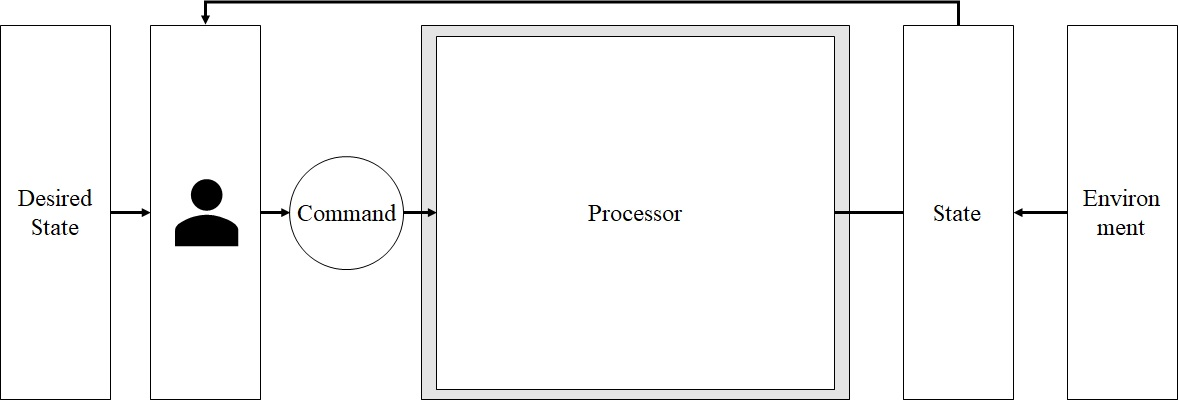
\includegraphics[clip,width=140mm]{images/imperative-system.jpg}}
    \caption{手続き型システム}\label{fig1}
\end{figure}

手続き型システムでは,あるべき状態(Desired State)に至る手続きをユーザが記述し,実行(Command)する.Commandを契機に,管理対象をあるべき状態へと操作する機能をProcessorと呼ぶ.

管理対象の状態(State)はProcessorからの操作だけでなく,環境(Environment)の影響も受けて変化する.故障や管理対象へのProcessorを介さない直接的な作業がその例である.したがって,ユーザは実行する際に改めて管理対象の状態を確認し,あるべき状態に至る手続きを調整する必要がある.そして,Processorが実行されない間に管理対象が環境の影響を受ければ,StateとDesired Stateには差が生まれる.つまり,Processorの実行から時間が経つにつれて,あるべき状態から離れていく.

\begin{figure}[h]
    \centerline{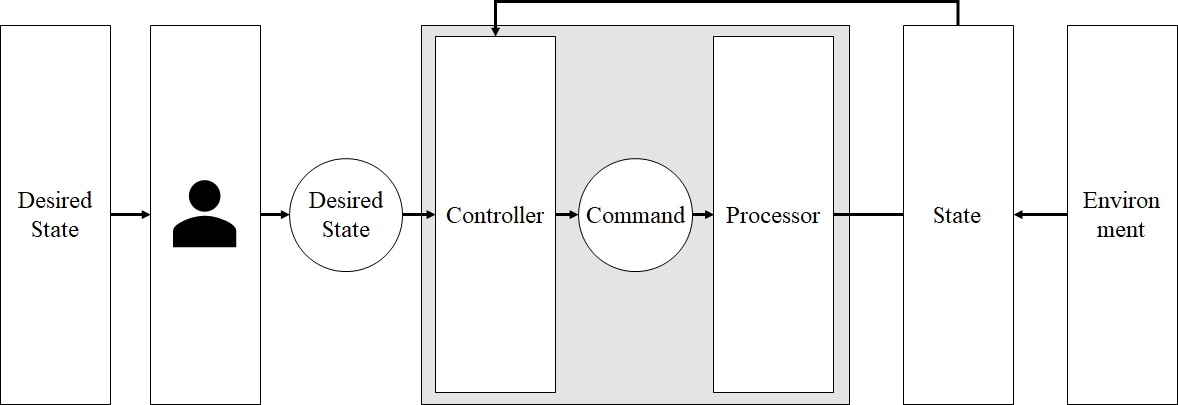
\includegraphics[clip,width=140mm]{images/declarative-system.jpg}}
    \caption{宣言型システム}\label{fig2}
\end{figure}

一方で宣言型システムでは,ユーザが記述し,システムへ入力するのは手続きではなく,あるべき状態である.つまり,あるべき状態を宣言する.そして,手続き型システムにおいてユーザが行っていた管理対象の状態確認とProcessorの実行は,Controllerが行う.Controllerが自動的,定期的に実行されれば,ユーザが明示的に実行せずとも,あるべき状態が維持される.

分散コンピューティング環境,特に大規模な基盤では常に構成要素のいずれかが故障している.また,基盤は環境の影響を受け,計画時に意図した構成から離れていく.運用者は多様で多数ある管理対象の状態を常に考慮して作業を行わねばならず,負担となっている.よって宣言と状態を分離し,状態を意識することなく,あるべき姿を維持できれば,その仕組みには価値がある.

宣言的システムは新しい概念ではないが,これまで分散コンピューティング基盤への適用には様々な課題があった.しかし,コンテナのスケジューリングや関連リソースの割り当てなど,オーケストレーションを実現するオープンソースソフトウェアであるKubernetes\cite{ref5}は,コンテナの特徴を活かし,結果整合を認めることで宣言的構成管理を実現した.特に構成管理と回復機能を一体にした構造は特徴的である.

反面,普及と同時に課題も散見され,Kubernetesコミュニティではサービス停止やアクシデント事例が数多く共有されている\cite{ref6}.宣言的構成管理というアイデアが普及する過程で明らかになった課題は示唆に富む.

\section{本論文の目的}
Kubernetesの回復性については,コンテナの回復時間に注目した先行研究\cite{ref7}があるが,構造上の特徴は追究されていない.また,Kubernetes自身が分散システムであり,開発も複数のグループに分かれているせいか,構造を俯瞰した情報が乏しい.CNCF(Cloud Native Computing Foundation)が2020年に行った調査\cite{ref8}では,コンテナの利用における課題として回答者の41\%がその複雑さを挙げている.これは回答の中で筆頭である.Kubernetesの全体構造を理解するために助けとなる情報の不足が,複雑さを感じる原因の1つと考える.

そこで本論文は,宣言的構成管理の先行例であるKubernetesの回復性を支える構造の分析を通じ,回復機能と一体である構成管理機能の構造上の特徴と課題を考察する.そして,本論文はKubernetesにとどまらず,宣言的構成管理を他の分散コンピューティング基盤へ適用する際に,検討や判断の助けになることを目的とする.よって構造分析と課題の抽出,その評価だけでなく,将来に向けての論点や展望も述べる.

\section{本論文の構成}
本論文は,まず第2章で本研究に関連する先行研究とその課題を整理し,Kubernetesがそれらを解決したアプローチを述べる.第3章で,STPAを用いたKuberntesの安全性,構造分析を行い,アクシデントにつながるハザードシナリオを識別する.第4章では,識別したハザードシナリオを障害事例によって分類し,その妥当性を評価する.第5章では,分析によって得られた構造上の特徴をもとに,宣言的構成管理を分散コンピューティング基盤へ適用する際に検討すべき論点や課題を述べる.第6章は,第5章の論点を踏まえ,宣言的構成管理の将来に向けた展望を考察する.最後に第7章で,本論文の成果と意義を述べる.

\chapter{関連研究と実装例}

\section{宣言的構成管理の課題}
宣言的構成管理はネットワークやクラウドコンピューティング領域で先行研究が存在する\cite{ref1,ref9,ref10}.そして,それらの基礎にはProlog\cite{ref11}など宣言型の制約,論理プログラミングがある.しかし,このコンセプトが一般化したとは言いにくい.

先に挙げた研究\cite{ref1,ref9,ref10}は2006年から2011年に発表されており,その時期はクラウドコンピューティングの普及初期である.だが,のちにクラウドコンピューティングの活用が進む一方で,宣言的構成管理の研究では特筆すべき進展はなかった.

なお,クラウドコンピューティングの普及に合わせ,リソースをAPIで操作可能な基盤が増えたことや,需要に応じて作成と削除を行いコストの最適化ができる利点などを背景に,プロビジョニング,構成を自動化するツールは一般的となった.

その中にはAnsibleやTerraformなど,管理対象リソースをYAMLなどのフォーマットで宣言的に表現可能なものもある.しかし,それらのツールは実行タイミングにおいてのみ,宣言をリソースへ適用する.稼働中のリソースを宣言した状態へと継続的に維持するには至っていない.Morrisはサーバの構成管理において,宣言と現状の差が広がらないよう,それらのツールの定期的な実行を推奨している\cite{ref12}.しかし,障害からの回復においては,手作業や,検知から回復を自動化する他の仕組みが必要とも指摘している.

もっとも,クラウドコンピューティングの多くは事業者のサービスとして提供されており,その管理手法のすべては明らかではない.しかし,仮に事業者が宣言的構成管理に関する取り組みや知見を公にしていないとしても,それのみが一般化を阻む要因ではないと考える.

分散コンピューティング基盤の構成に関わる条件やルール,制約を宣言し,適用し続けるアプローチが一般化しなかった理由を以下に考察する.

\subsection{管理対象が持つ自律性との齟齬}
構成管理機能と管理対象自身が持つ構成維持,回復機能が衝突する,もしくは過敏に反応することがある.また,構成管理機能ではトランザクション処理が可能であっても,管理対象がその境界外で非同期に動作するケースもある.

この齟齬を,Chenらはネットワークにおける宣言的構成管理の適用に関する研究で指摘している\cite{ref9}.例えば,ルーティングプロトコルやルータが故障や輻輳を検知し経路を切り替え,収束を待つ間に,構成管理機能から変更を指示すると,順序やタイミングによっては一時的なループや経路振動など不安定な状態に繋がる恐れがある.

またChenらは,管理対象に対して制約を適用している途中で,新たな制約が入力された場合の制御の難しさも挙げている.適用中の制約をロールバックし,新たな制約を含めて構成を再決定した上で,改めてトランザクションを実行する案が示されている.しかし,この案もネットワークの状態やタイミング次第で不安定な状態を生み出す要因となりうる.トランザクションによる解決の他に,管理対象からのフィードバックを評価する頻度,間隔の調整なども考慮すべきだろう.

なお分散コンピューティングでは,ユーザやアプリケーションが構成要素の位置や規模,障害などを意識せずに済むよう,透過性の担保が課題となる.その際,構成管理機能から管理対象を透過に操作するために,中間層を設けて抽象化するデザインが一般的である.分散コンピューティング基盤のリソース管理においては,サーバ上のリソースなど状態を部分,単一の要素で宣言,評価できる管理対象向けの中間層はシンプルに実装できるが,ネットワークサービスなど全体,エンドツーエンドで評価すべきものに対しては複雑になりやすい.加えて多重障害など状態とその組み合わせは多様であり,透過性担保のために中間層が肥大化,多層化する懸念がある.

\subsection{リソース操作に要する時間}
アプリケーションとは異なり,基盤を構成するリソースの中には状態の変更に時間を要するものがある.例えばクラウドコンピューティングサービスで仮想マシンの作成には一般的に数十秒を要する\cite{ref13}.宣言的構成管理において,仮想マシンがクラッシュした場合には宣言した数を維持するため再作成が必要だが,その間の数十秒は制約に反することになる.解決のために予備リソースを常時待機させる解決策もあるが,コストと複雑度は増す.

\subsection{構成の決定に要する時間と計算量}
リソースの操作だけでなく,その設定値を決定するのに要する時間と計算量も課題である.仮想スイッチのコントローラはその典型的な例である.コントローラは仮想マシンの作成やマイグレーションなどのイベントに追従し,宣言したポリシやルールに基づきフローを計算した上で,仮想スイッチへフローを配布する.管理対象の仮想スイッチ数に応じて計算量は増加し,拡張性を阻む要因となる.

この課題を解決するためには,イベント発生時に全体を再計算せず変化対象のみを計算し,変更が必要な管理対象にのみ配布するなどの考慮が必要となる.そこでRyzhykらは,PrologのサブセットであるDatalog\cite{ref14}を拡張し,ルールの差分評価に特化したDifferential Datalogで解決を試みている\cite{ref15}.型システムなど開発容易性も重視しており,後述する専門性に関する課題も合わせて解決しうるが,初版(v0.1)の公開が2019年と若いプロジェクトであり,現時点で本格化には至っていない.

\subsection{ポリシやルールの記述に必要な専門性}
先行研究ではポリシやルールを表現するために,先に挙げたDifferential Datalogの他に,Prologを元にしたCOPElog\cite{ref1}やNetwork Datalog\cite{ref10}が提案されている.制約,論理プログラミングの習得には専門性を必要とする.反面,宣言的構成管理が解決したい問題の1つは,専門性を持つ技術者への依存を解決することである.

\subsection{稼働中の基盤に変更を加えるリスク}
加えて稼働中の基盤に変更を加える影響とリスクが大きいことも,一般化を阻む要因であろう.例えばクラウドコンピューティングサービスの主な停止原因は変更作業である\cite{ref16}.多くのユーザが共用し,停止の影響が大きな基盤では変更作業を慎重に行わざるをえない.

宣言的構成管理においては,基盤のリソースを操作可能な,強い権限を管理アプリケーションに対して付与する.自動化によって時間あたりに操作可能なリソース量はスケールするが,反面,それを実現するアプリケーションに不具合があった場合の影響範囲も広くなる.

\section{Kubernetesの解決アプローチ}
しかし昨今,宣言的な構成管理を行う分散コンピューティング基盤としてKubernetesが注目され,導入例が増えている.CNCFが2020年に行った調査\cite{ref8}では回答者の91\%がKubernetesを導入しており,その内の83\%が本番環境で利用している.2018年の同調査では58\%であった.Kubernetesに対する関心が高いコミュニティでの調査ではあるが,活用の進展が読み取れる.

\subsection{Kubernetesの構造上の特徴}
図\ref{fig3}がKubernetesを構成する要素の概観である.Kubernetesの主な管理対象はコンテナであり,複数のコンテナを包含するPodを管理の単位とする.そして利用者はPodと関連リソースの仕様を宣言し,Kubernetesはそれを作成,維持する.なおKubernetesクラスタの土台となるサーバ,ネットワーク,ストレージなどインフラストラクチャの管理はKubernetesから分離されている.インフラストラクチャが提供するAPIを通じて操作は可能であるが,拡張機能であり選択は任意である.

\begin{figure}[tb]
  \centerline{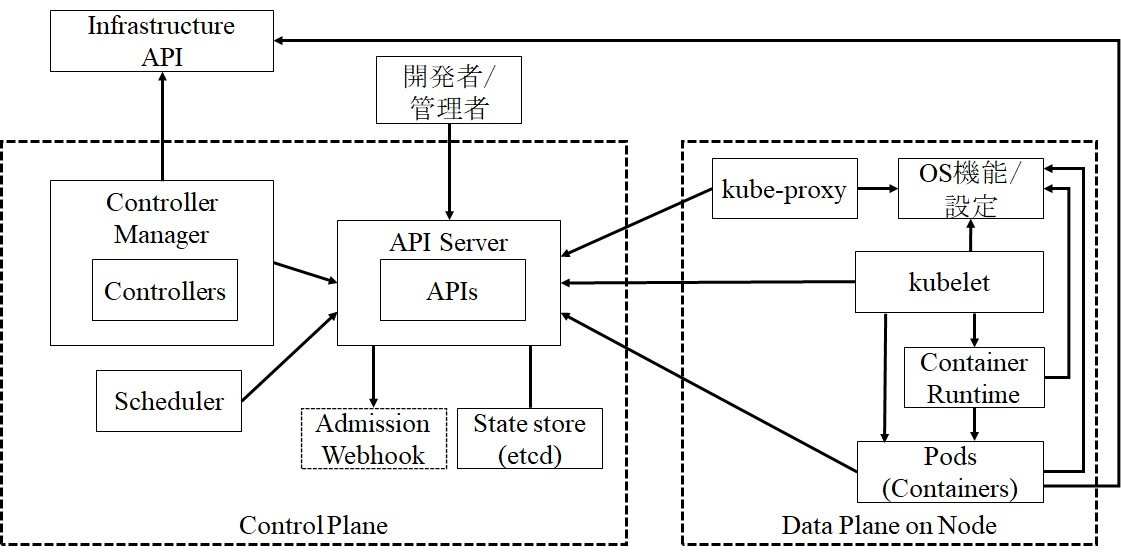
\includegraphics[clip,width=140mm]{images/k8s-overall.jpg}}
  \caption{Kubernetesの構成要素}\label{fig3}
\end{figure}

API Serverと状態ストア(etcd)が,Kubernetesリソースの宣言と状態を一元管理する.そしてリソースの種類毎にあるコントローラ群(Controller Manager)と,Podの配置先Nodeを決定するSchedulerが,API Serverを通じてリソースの構成情報,状態を操作する.本論文では,この範囲をコントロールプレーンとする.

また,Nodeはベアメタルサーバや仮想マシンで構成され,Podが動作する.Node上のkubeletがPodの定義に従い,コンテナランタイムを通じてコンテナや関連リソースを作成する.そして,kube-proxyはNodeのネットワーク設定やパケット転送を行う.この範囲はデータプレーンとする.

API Serverにアクセスするコントローラやkubeletなどの非API Server要素は,リソース作成,変更などイベント発生時にのみ動作するのではく,常に宣言と状態の差分を確認し,差分があれば埋める(Reconcile)よう一定間隔でループする(Control Loop).このロジックは共通クライアントライブラリ(client-go)に実装されており,以降で説明する非API Server要素はこれを利用するものとする.

操作の方向はAPI Serverからのプッシュではなく,非API Server要素からのプルである.また,API Serverへ問い合わせ,リソースの構成情報を更新するのは非API Server要素の責務である.そして,非API Server要素はそれぞれが担当するリソース固有の操作ロジックを持つ.一方,API Serverは反応的で,非API Server要素へデータを提供する順序やタイミングを制御しない.

非API Server要素は自身が担当するリソースのAPIからリソースの一覧を取得し(List),取得したリソースのイベントを監視する(Watch).WatchではHTTPヘッダのTransfer-Encodingをchnkedに設定しGETする.この操作によりHTTPコネクションを維持し,リソースの追加や変更,削除イベントが発生したタイミングで変化の内容を取得できる.そして,非API Server要素はリソース状態のキャッシュを持ち,API Serverの負担を軽減するが,定期的にAPI Server上の状態と同期する.

このようにKubernetesの非API Server要素はControl Loopで定期的にAPI Serverへ問い合わせを行い,一時的な通信断や遅延で要求が失敗しても.一定間隔で修正し続ける.つまりポーリングによって定期的に状態を確認,操作するレベルトリガ方式を採用している.加えて,イベントが発生したタイミングでも変更を受け取る.これはイベントを操作の契機とするエッジトリガとも言える.非API Server要素はレベルトリガとエッジトリガを組み合わせ,エラー耐性と即時性を両立している[図\ref{fig5}].

\begin{figure}[b]
    \centerline{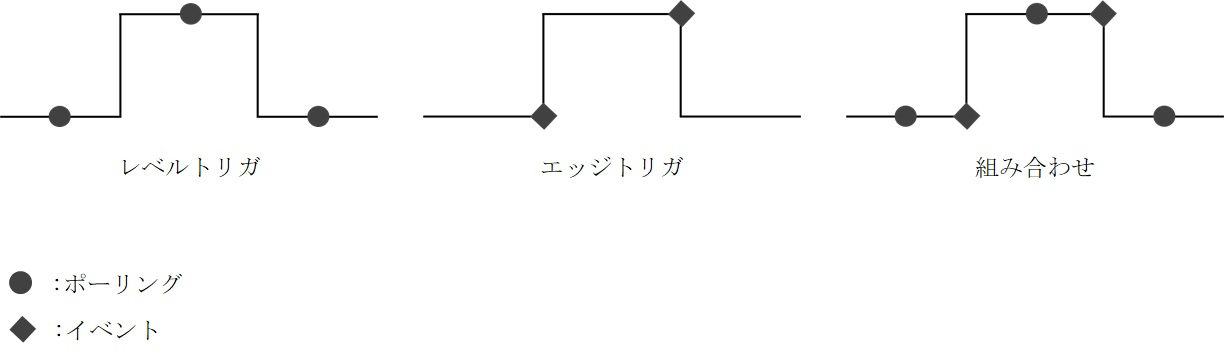
\includegraphics[clip,width=140mm]{images/trigger.jpg}}
    \caption{レベルトリガとエッジトリガ}\label{fig5}
\end{figure}

前述の通り,Kubernetesはリソースの種類毎にコントローラを持つ.そしてリソースの中には,複数の種類のリソースを組み合わせて構成されるものもある.そのようなリソースの管理には,複数のAPIとコントローラが関わる.例えば,Podの上位リソースには,Podのレプリカを管理するReplicaSetがある.そしてReplicaSetの上位に,ReplicaSetの更新やロールバックなどリリース管理を行うDeploymentがある.ソースコード\ref{sc1}は,Deploymentの宣言(マニフェスト)の例である.

\newpage
\begin{lstlisting}[caption=Deploymentの宣言例,label=sc1]
apiVersion: apps/v1
kind: Deployment
metadata:
  name: nginx-deployment
  labels:
    app: nginx
spec:
  replicas: 3
  selector:
    matchLabels:
      app: nginx
  template:
    metadata:
      labels:
        app: nginx
    spec:
      containers:
      - name: nginx
        image: nginx:1.14.2
        resources:
          limits:
            cpu: "1"
            memory: "100Mi"
          requests:
            cpu: "0.5"
            memory: "50Mi"
        ports:
        - containerPort: 80
\end{lstlisting}

.kindに最上位リソースであるDepoloymentを指定し,加えて下位リソースに必要な属性も宣言する.ソースコード\ref{sc1}ではReplicaSetの作成に必要なレプリカ数を.spec.replicasに,Podに必要なコンテナの属性を.spec.templateに宣言している.

Kubernetesの各要素は,自らが責務を持つリソースのAPIをList \& Watchし,イベントに合わせて下位リソースの作成など必要な操作を行う.つまり,複数のリソースを組み合わせたリソースの操作ではイベントが連鎖する.図\ref{fig4}はDeployment作成のイベントチェーンである.

\newpage
\begin{figure}[tb]
    \centerline{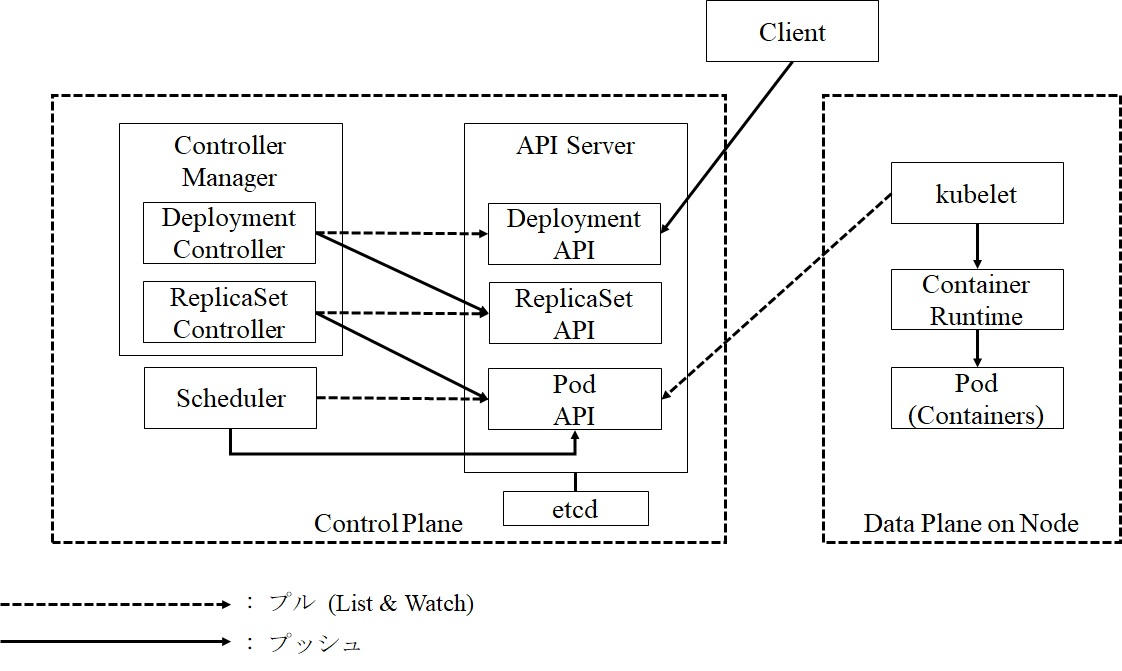
\includegraphics[clip,width=140mm]{images/k8s-event-chain.jpg}}
    \caption{Kubernetesのイベントチェーン(Deployment作成時)}\label{fig4}
\end{figure}

この例でわかるように,各コントローラは自身が責務を持つリソースを,イベントの発生や定期的なループを契機に,宣言した状態に収束させること,および直に接する下位リソースの操作に専念する.チェーン全体の制御は行わない.

ソースコード\ref{sc2}は,Tornowらが示したDeployment ControllerのControl Loopのアルゴリズム(PlusCal)である\cite{ref17}.

\newpage
\begin{lstlisting}[caption=Deployment Controllerのアルゴリズム,label=sc2]
process Controller = "Deployment Controller"
begin
  ControlLoop:
    while TRUE do
      \* The Deployment Controller monitors Deployment Objects
      with d ∈ {d ∈ k8s: d.kind = "Deployment"} do
        \* 1. Enabling Condition
        if Cardinality({r \in k8s: r.kind = "ReplicaSet" ∧ match(d.spec.labelSelector, r.meta.labels)}) < 1 then
          \* Reconciling Command
          CREATE([kind |-> "ReplicaSet", spec |-> [replicas |-> d.spec.replicas, template |-> d.spec.template]]);
        end if;
        \* 2. Enabling Condition
        if Cardinality({r \in k8s: r.kind = "ReplicaSet" ∧ match(d.spec.labelSelector, r.meta.labels)}) > 1 then
          \* Reconciling Command
          with r ∈ {r \in k8s: r.kind = "ReplicaSet" ∧ match(d.spec.labelSelector, r.meta.labels)} do
             DELETE(r);
          end with;
        end if;
      end with;
    end while;
end process;
\end{lstlisting}

Deployment Controllerはリソースの種類がDepolymentであるオブジェクトをControl Loopで監視し,labelが合致するReplicaSetの数を確認する.そして宣言と現状のレプリカ数に差分があれば増減を行う.\\

このような特徴を持つKubernetesであるが,支持を得た理由を宣言的構成管理の文脈で考察する.

\subsection{構成管理と回復機能が一体}
Kubernetesにおいて,宣言を満たすリソースの割り当てや設定と,故障や不具合からの回復は同じ機能で実現される.つまり一体である.よって構成管理と回復機能の齟齬が生じにくい.

また,Kubernetesが管理対象とし,操作するのはコンテナやiptablesなど,主にサーバの提供する機能やパラメータである.そして,リソース操作の主体となるkubeletやkube-proxyの責任範囲は自Nodeのみであり,他Nodeやネットワークの状態を意識しない.加えて,管理対象にルーティングプロトコルのような自律性もない.よって管理対象の透過性を担保するための仕組みをシンプルにできる.

なお前述の通り,クラウドサービスなどKubernetesの土台となる基盤が提供するAPIを通じてネットワーク,ストレージなどのリソースを操作する構成も可能であり,この場合は管理対象が自律性を有する場合もある.また,サーバOSの持つ汎用的な機能だけでなく,用途により特化,最適化されたリソースを活用したいというニーズも高まっている.例えば,CNI(Container Network Interface)\cite{ref18}やCSI(Conteiner Storage Interface)\cite{ref19}プロジェクトでは活発に議論,開発が行われている.管理対象リソースの広がりについては,改めて展望の章で述べる.

\subsection{リソース操作に要する時間が短い}
従来は仮想マシンの作成にかかる時間が課題であったことに対し,Kubernetesで主な操作対象はコンテナとそれを包含するPodであり,イメージのサイズや事前配備など条件を整えれば1秒以内で作成できる\cite{ref20}.また,MicroVMなど他の軽量な選択肢も増えている\cite{ref21}.これらの手段により,構成変更や回復が必要なタイミングでPodを再作成するというシンプルな戦略が可能となった.またネットワーク設定に関しても,操作対象がネットワーク全体や複数ノードではなく,iptablesなど単一Nodeでの操作であれば短時間で完了する.

なお操作の元となる設定を決定する時間や計算量については,規模と条件によっては課題がある.例えばNodeやPodの数が多い環境でAffinity制約を指定した場合に,SchedulerがPodの配置先の決定に時間を要することがある\cite{ref22}.

\subsection{結果整合の許容}
Kubernetesは宣言を受け付ける際,プラグイン可能なアドミッションコントロールなど例外を除き,入力内容の妥当性検証を行わない.例えば要求されたリソースに対し割り当て可能なものがなくとも,API Serverは拒否せず受け付け,利用可能なリソースが追加されるか空くのを待つ.リソースの入力時,複雑な検証アルゴリズムやその計算にかかる待ち時間を不要とした.

また,ネットワークを介して接続される分散システムでは,管理対象の正確な状態把握は困難である.そこでKubernetesの各要素はAPI Serverから得られる状態(Current State)を正とし,仮に実際の状態(Actual State)と異なっていても,一時的な不整合を受け入れ,Control Loopで解決する\cite{ref23}.

なお,多様な要素がAPI Serverを通じてリソースの状態を参照,操作するKubernetesにおいて,並行性制御の戦略は重要である.仮に悲観的並行性制御を採用し,ロックを前提に実装すると,規模の拡張性が課題となりやすい.そこでKubernetesは,ロックを用いない楽観的並行性制御を採用している.各リソースはバージョン情報を持ち,APIのクライアントはリソースの更新を要求する際に,自身が把握しているバージョンを示す.API Serverは更新要求を受け取ると,リソースの現在のバージョンとクライアントが示したバージョンを比較する.そしてクライアントが示したバージョンが古ければ,別のクライアントがすでに更新したと判断し,更新を拒否する.しかし,拒否されてもControl Loopによって更新要求は再試行され,いずれ成功する.

なお,この楽観的並行性制御は,Kubernetesの原型であるOmegaで,拡張性を確保するために採用された\cite{ref24}.

\subsection{論理ではなく状態を記述}
ソースコード\ref{sc1}に示した通り,Kubernetesの利用者はリソースのあるべき状態をJSONやYAMLフォーマットで宣言する.リソースの属性を理解する必要はあるが,制約やルールをプログラミングする必要はない.構成をコードではなくデータで記述できる(Configuration as Data)\cite{ref25}とも言える.かつ,その抽象度は高くなく,Podに必要なリソースの量やレプリカの数,起動や配置条件など属性を直接的に記述できる.

\chapter{提案手法}

\section{STPAを選択した理由}
Kubernetesの構成要素は多様で,相互に作用する.よって各構成要素が期待通りに動作しても,構成要素の内部状態や受け渡されるデータによっては,全体として問題が生じる可能性がある.つまりKubernetesの安全性分析では,構成要素単体の故障や不具合に注目すると特徴を捉えられない.そこで本論文では,事故因果関係モデルSTAMP(System-Theoretic Accident Model and Processes)を基礎とするハザード分析手法STPA(System-Theoretic Process Analysis)\cite{ref26,ref27,ref28}を選択する.

STPAにおいて損失は構成要素の相互作用の結果と考えるため,Kubernetesの安全性分析に適する.また,STPAでは分析過程で制御構造図(コントロールストラクチャ)を成果物とするが,構造上の課題の考察に有用である.

\section{分析目的の定義}
STPAの本来の目的は人命,設備,金銭などの損失を防ぐことである.損失の重要度や影響の大きさはシステムの位置づけと利害関係者に依存するため,まず目的を定義する.はじめに受け入れられない損失を定義し,損失に繋がるシステムの状態や条件であるハザードを識別する.本分析では一般的なビジネスアプリケーションを想定し,顧客満足の喪失を受け入れられない損失とする[表\ref{table1}].そしてハザードは顧客満足を得て維持するために必要なサービスレベルを満たせていない状態とし,高遅延,タイムアウト,エラー応答の発生とした.具体的な数値は割愛する.

最後に,ハザードを防ぐために満たすべきシステムの条件や動作である安全制約を定義する.本分析はKubernetesがPodを安全に動かすために守るべき制約に焦点を絞る.
\newpage
\begin{table}[t]
    \centering
    \caption{分析目的の定義}\label{table1}
    \begin{tabularx}{\linewidth}{X|X|X}
        損失           & ハザード          & 安全制約                                                                                                      \\ \hline \hline
        顧客満足の喪失 & H-1: 高遅延       & SC-1: Podが必要とする機能を提供,維持しなければならない(ConfigMapや名前解決など) [H-1, H-2, H-3]              \\ \cline{3-3}
                       & H-2: タイムアウト & SC-2: Podに適切な量の資源を提供,維持しなければならない(CPU,メモリなど) [H-1, H-2, H-3]                      \\ \cline{3-3}
                       & H-3: エラー応答   & SC-3: Podがサービス提供するのに必要なクラスタ内ネットワーク経路を提供,維持しなければならない [H-1, H-2, H-3] \\ \hline
    \end{tabularx}
\end{table}

なお分析の対象範囲はKubernetesクラスタとその上で動作するアプリケーションとする.よって,例えばユーザからクラスタに至るネットワーク経路などは範囲外である.

\section{コントロールストラクチャの図式化}
分析目的の定義に続き,要素間の制御とフィードバックの流れを可視化するため,コントロールストラクチャを作成する.まずシステム全体を概観し特徴を得る[図\ref{fig6}].
\newpage
\begin{figure}[tb]
    \centerline{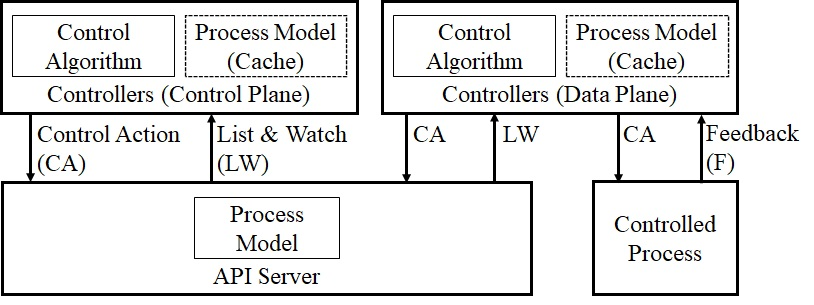
\includegraphics[clip,width=140mm]{images/cs-system.jpg}}
    \caption{コントロールストラクチャ(システムレベル)}\label{fig6}
\end{figure}

STPAでは被コントロールプロセスの状態など,コントローラが信じていることをプロセスモデルと呼ぶ.KubernetesではAPI Serverがプロセスモデルを一元的に管理している.

各コントローラはプロセスモデルのキャッシュを持ち,API Serverの変化イベントを監視する.加えて,Control Loopで定期的にチェックする.そして宣言と状態に差分が生じた場合に,それぞれの責務にしたがって処理を行う.

プロセスモデルが一元管理され,継続的に問い合わせと更新を繰り返すため,分散システムで課題となりがちな,不適切なプロセスモデルやフィードバックを原因とする問題が起きにくい.仮に更新が一時的に滞ったとしても,いずれAPI Server上のプロセスモデルと同期されるからである.

次に,各コントローラの制御動作であるコントロールアクションを識別するため,サブシステムレベルのコントロールストラクチャを作成する[図\ref{fig7}][図\ref{fig8}].

ただし要素間の相互作用と構造上の安全性分析が目的であるため,各要素は冗長化され,単一故障に耐えると仮定する.同様に,各要素のコントロールアルゴリズムは適切とする.

なお図式化によりトレーサビリティがあるため,複数のコントローラの作用の結果生じるハザードは,ハザードの直接的な原因となったコントロールアクションのみを識別する.そして簡単のため,要素間に複数のコントロールアクションがある場合,1つの識別子にまとめる.
\newpage
\begin{figure}[tb]
    \centerline{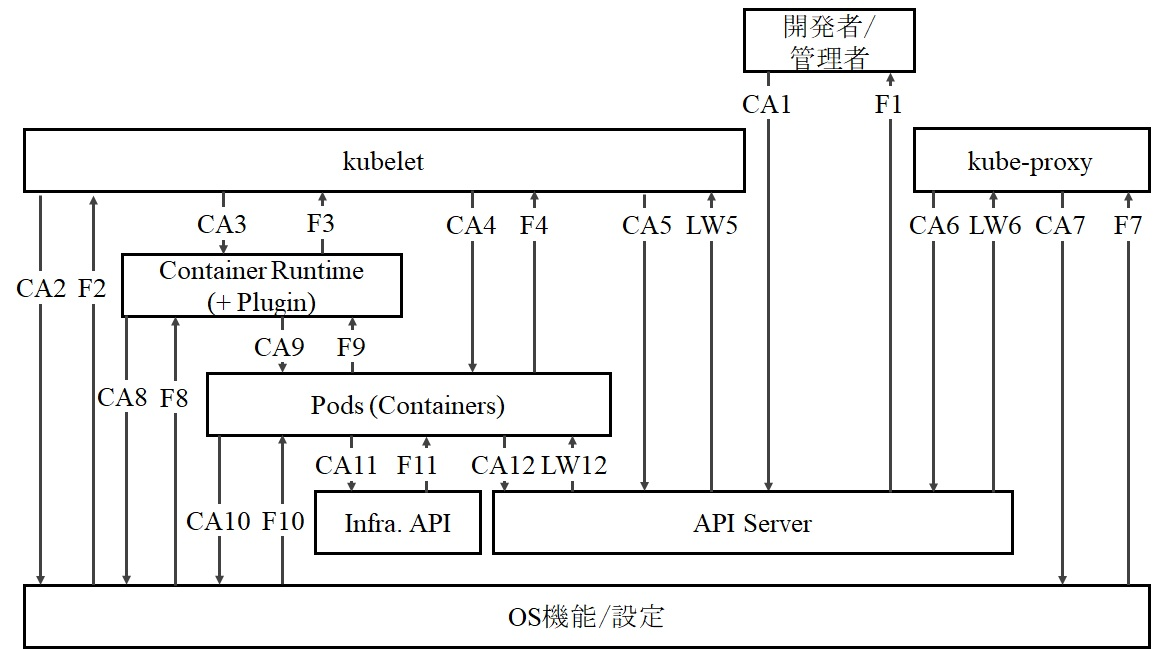
\includegraphics[clip,width=140mm]{images/cs-dataplane.jpg}}
    \caption{コントロールストラクチャ(データプレーン)}\label{fig7}
\end{figure}
\begin{figure}[h]
    \centerline{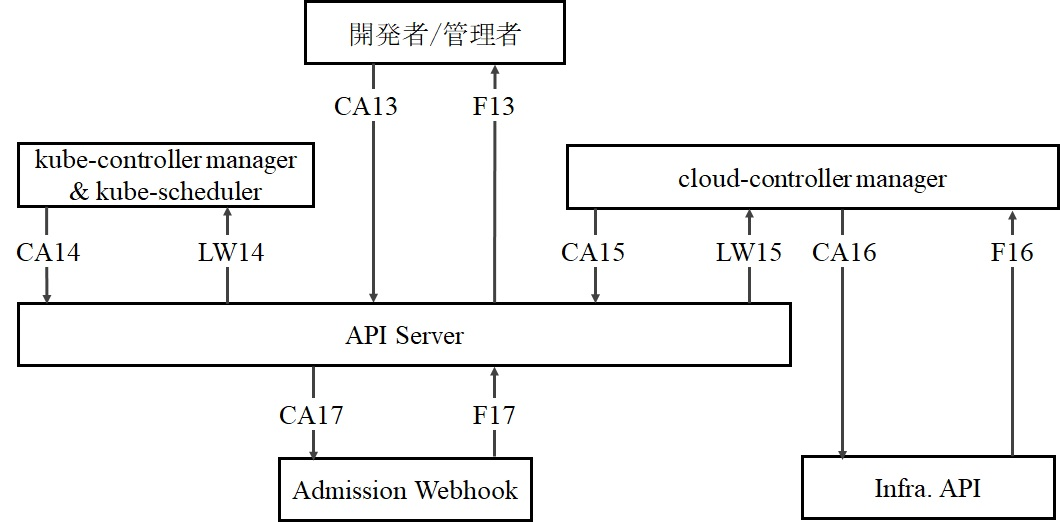
\includegraphics[clip,width=140mm]{images/cs-controlplane.jpg}}
    \caption{コントロールストラクチャ(コントロールプレーン)}\label{fig8}
\end{figure}

STPAのコントロールストラクチャでは権限の大きい,制御の起点となるコントローラを図の上部に配置する.そして,API Serverはコントロールストラクチャでは下部に位置付けられる.つまり,API ServerはKubernetesの中核機能でありながら,反応的な被コントロールプロセスであることが確認できる.

\section{非安全なコントロールアクションの識別}
次に,識別したコントロールアクションから,ハザードにつながる非安全なコントロールアクション(UCA: Unsafe Control Action)を識別する.識別には3つのガイドワード「与えられないとハザード」「与えられるとハザード」「早すぎ,遅過ぎ,誤順序」を活用する.

なお「早すぎる停止,長すぎる適用」もSTPAのガイドワードであるが,自動車のブレーキを踏み続けるような連続的なコントロールアクションを対象とするため,離散的なAPI呼び出しがコントロールアクションの大部分であるKubernetesの分析では適用しない.

識別した非安全なコントロールアクションの一覧を表\ref{table2}に示す.
\newpage
\begin{footnotesize}
    \begin{tabularx}{\linewidth}{
            >{\hsize=0.7\hsize}X|
            >{\hsize=1.1\hsize}X|
            >{\hsize=1.1\hsize}X|
            >{\hsize=1.1\hsize}X
        }
        \captionsetup{font=normalsize}
        \caption{非安全なコントロールアクション(UCA: Unsafe Control Action)一覧}\label{table2}                                                                                                                                                                                                                                                                                                                                                                                                                                                                                                                                                                                                                                                                                                                                                                                                                                                                                                                                                              \\
        コントロールアクション                                        & 与えられないとハザード                                                                                                                                                                                                                                                                                                                                                                                                                                                                                     & 与えられるとハザード                                                                                                                                                                                                                                                                                                            & 早過ぎ,遅過ぎ,誤順序                                                                                                               \\  \hline \hline
        \endfirsthead
        \multicolumn{4}{l}{前ページからの続き}                                                                                                                                                                                                                                                                                                                                                                                                                                                                                                                                                                                                                                                                                                                                                                                                                                                                                                                                                                                                              \\
        \hline
        コントロールアクション                                        & 与えられないとハザード                                                                                                                                                                                                                                                                                                                                                                                                                                                                                     & 与えられるとハザード                                                                                                                                                                                                                                                                                                            & 早過ぎ,遅過ぎ,誤順序                                                                                                               \\  \hline \hline
        \endhead
        \multicolumn{4}{r}{次ページに続く}                                                                                                                                                                                                                                                                                                                                                                                                                                                                                                                                                                                                                                                                                                                                                                                                                                                                                                                                                                                                                  \\
        \endfoot
        \multicolumn{4}{r}{表の終わり}                                                                                                                                                                                                                                                                                                                                                                                                                                                                                                                                                                                                                                                                                                                                                                                                                                                                                                                                                                                                                      \\
        \endlastfoot
        CA-3(kubelet から Container Runtime)                          & UCA-1: Podは正常に動作しているが,relist処理の遅延などで,そう判断されない.結果,NodeがNotReady状態と判断され,サービス提供に必要なリソースが減少する[H-1]                                                                                                                                                                                                                                                                                                                                                & UCA-2: ImagePullPolicy=Always設定で短時間に大量のコンテナを作成する.ネットワーク帯域の圧迫だけでなく,レジストリに拒否されPodが作成できない[H-1]                                                                                                                                                                               & -                                                                                                                                    \\ \hline
        CA-4(kubelet から Pod)                                        & -                                                                                                                                                                                                                                                                                                                                                                                                                                                                                                          & UCA-3: 敏感過ぎるliveness Probe設定によりPod再作成が頻発し,サービス提供能力が低下する[H-1]                                                                                                                                                                                                                                     & UCA-4: Readiness Probeの不備で準備不十分なPodへトラフィックが転送される[H-3]                                                         \\ \hline
        CA-5(kubelet から API Server)                                 & UCA-5: Nodeが正常な状態にも関わらず,API Serverに伝わらない.経路が問題の場合はクラスタ全体に影響が及ぶ.例えば,Node自動修復機能がNode作成と削除をクラスタ全体で繰り返す [H-1, H-2, H-3] \par\noindent                                                                                                                                                                                                                             UCA-6: 十分なAPI Server呼び出しレートが設定されていない[H-1, H-2, H-3] & UCA-7: API Serverが過剰に呼び出され,API Serverが過負荷状態に陥る[H-1, H-2, H-3]                                                                                                                                                                                                                                                & -                                                                                                                                    \\ \hline
        CA-7(kube-proxy から OS機能/設定)                             & UCA-8: iptables,conntrackなどIP転送に関する更新が行われない[H-3]                                                                                                                                                                                                                                                                                                                                                                                                                                          & -                                                                                                                                                                                                                                                                                                                               & UCA-9: IP転送に関する更新が要素やNode間で同期しない(IngressとServiceのEndpointなど)[H-3]                                   \\ \hline
        CA-8(Container Runtime から OS機能/設定)                      & UCA-10: サービス提供に必要なPodに十分なNodeのリソースや優先度が割り当てられない.リソース利用率が高まると強制終了される[H-1, H-2, H-3]\par\noindent UCA-11: 適切なSNATアルゴリズムなどサービスレベル遵守に必要な設定が行われない[H-1]                                                                                                                                                                                                                                                                      & UCA-12: サービス提供に貢献度の低いPodに過剰なNodeのリソースや高い優先度が割り当てられる.リソース利用率が高まるとサービス提供に必要なPodやNodeのプロセスが強制終了される[H-1, H-2, H-3]\par\noindent UCA-13: カーネルの監査ログ有効化などNode単位で影響する負荷の高い設定が行われる.Podに十分なリソースが割り当てられない[H-1] & -                                                                                                                                    \\ \hline
        CA-9(Container Runtime から Pod)                              & -                                                                                                                                                                                                                                                                                                                                                                                                                                                                                                          & UCA-14: 過剰なDNS問い合わせを行うよう設定される.例えば既定のndots: 5設定を見直していない[H-1, H-2, H-3]                                                                                                                                                                                                                        & -                                                                                                                                    \\ \hline
        CA-11(Pod から Infrastructure API)                            & UCA-15: Cluster AutoscalerによるNodeやボリューム追加などにおいて,サービスレベル遵守に必要なインフラリソースの作成指示が行われない[H-1]                                                                                                                                                                                                                                                                                                                                                                    & UCA-16: Podに割り当てられない,別データセンタでのボリューム作成など,不整合のあるリソースの作成指示が行われる[H-1, H-2, H-3]                                                                                                                                                                                                    & UCA-17: Cluster AutoscalerによるNode削除などにおいて,リソースの削除や割当解除の指示が早すぎる.設定した猶予時間が短すぎる[H-1, H-3] \\ \hline
        CA-12(Pod から API Server)                                    & UCA-18: サービスメッシュのOperatorなどシステム全体に影響の大きなPodからのコントロールアクションが行われない.関連する変更操作が停止する[H-1, H-2, H-3]                                                                                                                                                                                                                                                                                                                                                     & UCA-19: API Serverが過剰に呼び出され,API Serverが過負荷状態に陥る[H-1, H-2, H-3]                                                                                                                                                                                                                                               & -                                                                                                                                    \\ \hline
        CA-13(開発者や管理者 から API Server)                         & -                                                                                                                                                                                                                                                                                                                                                                                                                                                                                                          & -                                                                                                                                                                                                                                                                                                                               & UCA-20: ConfigMapやSecretはPod作成のタイミングで読み込まれるため,変更後に意図的に再作成しないとPod間で設定の不一致が生じる[H-3]     \\ \hline
        CA-14(kube-controller manager/kube-scheduler から API Server) & UCA-21: リソース作成のイベント(チェーン)が発生しない,もしくは途切れ,新規Podが作成されない[H-1, H-2, H-3]\par\noindent UCA-22: Podのスケジューリング結果が登録されず,新規Podが作成されない[H-1]                                                                                                                                                                                                                                                                                                          & UCA-23: Tolerationの指定漏れなどスケジュールできないPodやCronJobが大量に要求される.Pending状態の大量のPodがスケジューリング負荷の増大を招く[H-1]                                                                                                                                                                               & -                                                                                                                                    \\ \hline
        CA-15(cloud-controller manager から API Server)               & UCA-24: 作成したインフラリソースの情報が登録されず,利用可能と認識されない.処理量の増加に対応できない[H-1]                                                                                                                                                                                                                                                                                                                                                                                                & -                                                                                                                                                                                                                                                                                                                               & -                                                                                                                                    \\ \hline
        CA-16(cloud-controller manager から infra. API)               & UCA-25: 要求したインフラリソースが作成されない[H-1, H-2, H-3]                                                                                                                                                                                                                                                                                                                                                                                                                                              & UCA-26: 必要なインフラリソースが削除される[H-1, H-2, H-3]\par\noindent UCA-27: 利用可能量や制約,権限を超えたインフラリソースの作成が指示され,失敗する[H-1]                                                                                                                                                                    & -                                                                                                                                    \\ \hline
        CA-17(API Server から Admission Webhook)                      & UCA-28: Webhookが実行されず,Sidecarコンテナなどアプリケーションの依存するリソースがPodに注入されない[H-2, H-3]                                                                                                                                                                                                                                                                                                                                                                                            & UCA-29: Admission Controlの定義やポリシに適合しないリソースが要求され,失敗する[H-2, H-3]                                                                                                                                                                                                                                       & UCA-30: Webhook呼び出し先が準備できていない状態で実行される[H-2, H-3]                                                                \\ \hline
    \end{tabularx}
\end{footnotesize}

\section{ハザードにつながるシナリオ(要因)の識別}
分析の最後に,非安全なコントロールアクションに至る要因,シナリオを識別する.STPAにおけるシナリオにはタイプがあり,2つのグループに大別できる.

\subsection{非安全なコントロールアクションが起こる要因}
このグループにタイプは4つあり,「コントローラの故障」「不適切なコントロールアルゴリズムと実装」「非安全なコントロール入力」「不十分または不適切なプロセスモデル/フィードバック」である.

なお本分析では構造に注目するため,「コントローラの故障」と「不適切なコントロールアルゴリズムと実装」を除く.

\subsection{コントロールアクションが不適切に実行される,または実行されない要因}
もう1つのグループには2つのタイプがあり,「コントロール経路の問題」「被コントロールプロセスの問題」である.

非安全なコントロールアクションをこれらのタイプごとに整理し,シナリオを識別した[表\ref{table3}].
\newpage
\begin{footnotesize}
    \begin{tabularx}{\linewidth}{
            >{\hsize=1\hsize}X|
            >{\hsize=0.5\hsize}X|
            >{\hsize=2.0\hsize}X|
            >{\hsize=0.5\hsize}X
        }
        \captionsetup{font=normalsize}
        \caption{ハザードシナリオ一覧}\label{table3}                                                                                                                                                                                                                                                                                   \\
        タイプ                                        & 識別子 & シナリオ                                                                                                                                                                                                          & UCA                                               \\ \hline \hline
        \endfirsthead
        \multicolumn{4}{l}{前ページからの続き}                                                                                                                                                                                                                                                                                         \\
        \hline
        タイプ                                        & 識別子 & シナリオ                                                                                                                                                                                                          & UCA                                               \\ \hline \hline
        \endhead
        \multicolumn{4}{r}{次ページに続く}                                                                                                                                                                                                                                                                                             \\
        \endfoot
        \multicolumn{4}{r}{表の終わり}                                                                                                                                                                                                                                                                                                 \\
        \endlastfoot
        非安全なコントロール入力                      & HS-1   & 開発者や管理者が,Podに適切なリソース要求(Request)と制限(Limit),優先度設定(Priority Class),分離やNode特性に応じた設定(Taint/Toleration,Affinity/Anti Affinity)を行っていない.また,それを検証する仕組みがない & 10, 12, 23                                        \\ \cline{2-4}
                                                      & HS-2   & 開発者や管理者が,(HS-1に含まれない)Kubernetes要素の仕様や挙動,制約,状態,サイズを加味した設定や入力,実装を行っていない.また,それを検証する仕組みがない                                            & 2, 3, 4, 6 ,9, 11, 13, 14, 16, 17, 20, 23, 29, 30 \\ \cline{2-4}
                                                      & HS-3   & 開発者や管理者が,(HS-1, 2に含まれない)Nodeやインフラリソース,外部依存先の仕様や挙動,制約,状態,サイズを加味した設定や入力を行っていない.また,それを検証する仕組みがない                                     & 2, 11, 13, 16, 27, 30                             \\ \cline{2-4}
                                                      & HS-4   & 開発者や管理者が,サービス提供に必要なリソースを削除してしまう.また,それを検証する仕組みがない                                                                                                                  & 26                                                \\ \hline
        不十分,不適切なプロセスモデル/フィードバック & -      & -                                                                                                                                                                                                                 & -                                                 \\ \hline
        コントロール経路の問題                        & HS-5   & Data PlaneからAPI Serverへの経路が失われる,疎通できない                                                                                                                                                          & 5, 8, 18                                          \\ \cline{2-4}
                                                      & HS-6   & Control PlaneからAPI Serverへの経路が失われる,疎通できない                                                                                                                                                       & 21, 22, 24                                        \\ \cline{2-4}
                                                      & HS-7   & Data PlaneからInfra. APIへの経路が失われる,疎通できない                                                                                                                                                          & 15                                                \\ \cline{2-4}
                                                      & HS-8   & Control PlaneからInfra. APIへの経路が失われる,疎通できない                                                                                                                                                       & 25                                                \\ \cline{2-4}
                                                      & HS-9   & Control PlaneからPodやAdmission Webhookへの経路が失われる,疎通できない                                                                                                                                           & 28                                                \\ \hline
        被コントロールプロセスの問題                  & HS-10  & 被コントロールプロセスが長時間応答しない(過負荷によるフリーズやインフラ変更の待ち時間など)                                                                                                                      & 1                                                 \\ \cline{2-4}
                                                      & HS-11  & Data PlaneからAPI Serverへ過剰な数の要求が行われる(API Serverの能力とNode数が不均衡)                                                                                                                              & 7, 19                                             \\ \hline
    \end{tabularx}
\end{footnotesize}

注目すべきは,非安全なコントロール入力を要因とするシナリオの数である.アプリケーション開発者やシステム管理者の入力したリソース量などの宣言がハザード要因になっており,それを防ぐ仕組みが不十分と推測される.

一方で不十分,不適切なプロセスモデル/フィードバックを原因とするシナリオが無い.これはControl Loopによるプロセスモデルの継続的な更新と結果整合の許容という特徴から説明できる.

\chapter{評価}

\section{障害事例のハザードシナリオによる分類}
Kubernetesコミュニティで共有されている障害事例\cite{ref6}を参考に,識別したハザードシナリオを評価する.
原因を特定し,根拠が説明されている事例から,原因が本分析の対象範囲にある事例を抽出した.結果,本分析でSTPAにより識別したシナリオですべての事例を分類できた[表\ref{table4}].よって網羅性の観点で妥当と判断できる.

また,非安全なコントロール入力(HS-1,HS-2,HS-3)が支配的な要因であることが事例の数からもわかる.Kubernetesが結果整合を受け入れ,宣言の入力時検証を任意とした負の影響を認める.
\newpage
\begin{footnotesize}
    \begin{tabularx}{\linewidth}{
            >{\hsize=2.2\hsize}X|
            >{\hsize=0.5\hsize}X|
            >{\hsize=0.3\hsize}X
        }
        \captionsetup{font=normalsize}
        \caption{事例の原因とシナリオとの対応,数}\label{table4}                                                                                            \\
        原因                                                                                                                            & シナリオ & 事例数 \\ \hline \hline
        \endfirsthead
        \multicolumn{3}{l}{前ページからの続き}                                                                                                              \\
        \hline
        原因                                                                                                                            & シナリオ & 事例数 \\ \hline \hline
        \endhead
        \multicolumn{3}{r}{次ページに続く}                                                                                                                  \\
        \endfoot
        \multicolumn{3}{r}{表の終わり}                                                                                                                      \\
        \endlastfoot
        Podのリソース利用量にLimitを設定しておらずOOM Killやクラッシュが発生した                                                        & HS-1     & 6      \\ \cline{1-1} \cline{3-3}
        Priority Classの設定ミスで重要度の高いPodのPriorityが低く再作成対象となった                                                     &          & 2      \\ \cline{1-1} \cline{3-3}
        認証情報取得アプリケーションのメモリ利用量過多によりOOM KillとPod再作成が多発し,API Serverへの問い合わせが急増した             &          & 1      \\ \hline
        大量のDNS問い合わせによる名前解決の遅延,DNS稼働Nodeの過負荷,問い合わせ元Nodeのアウトバウンド通信過負荷                        & HS-2     & 6      \\ \cline{1-1} \cline{3-3}
        CronJob,Jobの設定ミスで大量のJobを実行,大量のPending Podによるスケジューリング過負荷,再実行ループの発生                      &          & 5      \\ \cline{1-1} \cline{3-3}
        Endpointの削除に時間を要し,Ingressが削除済みのPodにトラフィックを送信した                                                      &          & 2      \\ \cline{1-1} \cline{3-3}
        kubeletのAPI Server問い合わせレート制限が低過ぎ,認証情報の取得ができなかった                                                   &          & 2      \\ \cline{1-1} \cline{3-3}
        アップグレード時にOPAがAPI Serverの起動を拒否するポリシを適用し,API Serverが起動できなかった                                   &          & 1      \\ \cline{1-1} \cline{3-3}
        API Serverが利用できない状態でNodeの自動修復が機能し,Node再作成を繰り返した                                                    &          & 1      \\ \cline{1-1} \cline{3-3}
        監査ログがDisk I/Oを圧迫した                                                                                                    &          & 1      \\ \cline{1-1} \cline{3-3}
        イメージプル過多でレジストリが要求を拒否した(ImagePullPolicy=Alwaysを設定)                                                     &          & 1      \\ \cline{1-1} \cline{3-3}
        HPAとDeploymentのレプリカ数設定が合っていない                                                                                   &          & 1      \\ \cline{1-1} \cline{3-3}
        ConfigMap/Secretの変更後にPodを明示的に再作成せず,複数あるPodが異なる設定で動作した                                            &          & 1      \\ \cline{1-1} \cline{3-3}
        Node Pool移行時に旧Node PoolにEndpointが残存した(Drain漏れ)                                                                    &          & 1      \\ \cline{1-1} \cline{3-3}
        Pod Disruption Budgetを設定せずPodが一斉に再作成された                                                                          &          & 1      \\ \cline{1-1} \cline{3-3}
        敏感すぎるliveness proveでPodが頻繁に再作成された                                                                               &          & 1      \\ \cline{1-1} \cline{3-3}
        Cluster Autoscalerのスケールイン猶予時間が短過ぎ,急激にNode数が減少した                                                        &          & 1      \\ \hline
        アウトバウンド通信過多でconntrackテーブルが飽和,競合した                                                                       & HS-3     & 3      \\ \cline{1-1} \cline{3-3}
        CFSスケジューラの特性を理解せずCPU Limitを設定し,想定以上のスロットリングが発生した                                            &          & 1      \\ \cline{1-1} \cline{3-3}
        Node,Podともにオートスケール設定をしたが,仮想ネットワークのPod IP仕様を誤解し,IPアドレスを割り当てられず,スケールに失敗した &          & 1      \\ \cline{1-1} \cline{3-3}
        CNIのSNAT設定が不適切であり,割り当てられるポートが不足した                                                                     &          & 1      \\ \cline{1-1} \cline{3-3}
        PVが存在しない/別データセンタにありPodを起動できなかった                                                                        &          & 1      \\ \cline{1-1} \cline{3-3}
        起動コンテナ数が過多でファイルディスクリプタが枯渇した                                                                          &          & 1      \\ \hline
        Pod Lifecycle Event Generator relistなどコンテナランタイムの処理がタイムアウトしNodeがNotReady状態となった(過負荷など)         & HS-10    & 2      \\ \hline
        多Node環境においてDaemonSetからのAPI呼び出しがAPI Serverの過負荷につながった                                                    & HS-11    & 1      \\ \hline
    \end{tabularx}
\end{footnotesize}

\chapter{論点}

\section{入力時検証}
識別したハザードシナリオと事例が示す通り,宣言の入力時検証は明らかな論点である.なおKubernetesコミュニティは必要性の高まりから,Open Policy Agentプロジェクト\cite{ref29}で,ポリシベースの入力値検証機能を開発している.

ただし現状の厳密な把握を前提に,受け入れ可能な入力値を検証することには議論がある.その実現には低遅延なテレメトリが求められる.また,過度に現状を求めることは結果整合を許容して得た利点と相反するため,トレードオフを踏まえた判断が必要である.

\section{アプリケーションの再構成耐性}
\label{sec:アプリケーションの再構成耐性}
Kubernetesのように,構成管理を行う要素が非同期に並行動作する構造では,依存関係のある管理対象の間で設定に一時的な不整合が生じうる.

例えばKubernetesではPodの削除とEndpointからのPodの削除は並行して行われる.図\ref{fig9}からもわかる通り,Podを削除する際,PodがEndpointより先に削除される可能性がある.この間にクライアントがServiceへアクセスすると,Endpointリストの中から削除済みPodのIPアドレスが選択され,コネクションが拒否,リセットされる恐れがある[表\ref{table2}: UCA-9].図\ref{fig9}はパケット転送とその設定にkube-proxyとiptablesを利用する例であるが,他の方式でもEndpoint APIをWatchするものであれば同様である.Podの削除と再作成は構成変更の基本戦略であり,Nodeのメンテナンスやアプリケーションのバージョンアップなどにおいて日常的に発生する,軽視できない挙動である.以下にPodの削除や再作成を伴うイベントや作業の例を挙げる.なお,故障に関連するものは除く.

\begin{itemize}
  \item アプリケーションの更新
  \item 処理能力の拡張,縮小に伴うレプリカ数の自動/手動増減
  \item Nodeのメンテナンスに伴う排出と他Nodeでの再作成
  \item Node追加,削除に伴うリバランス
  \item リソース不足に伴うNodeからの強制排出と他Nodeでの再作成
\end{itemize}

\newpage
\begin{figure}[tb]
    \centerline{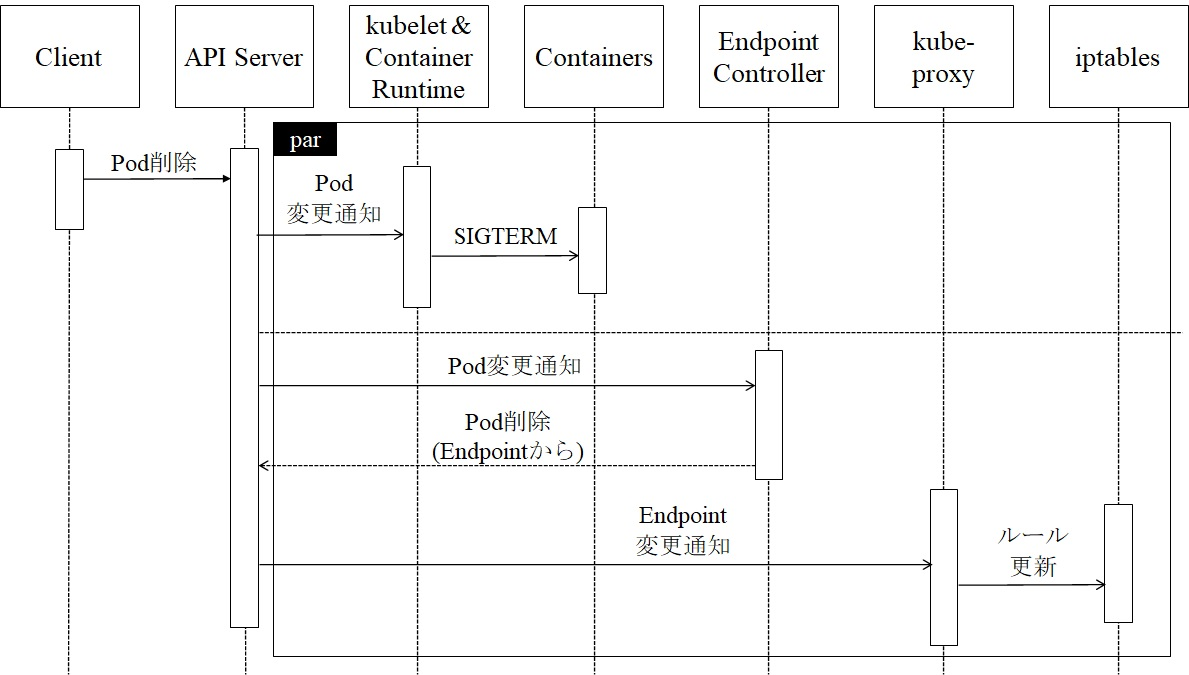
\includegraphics[clip,width=140mm]{images/del-pod-sequence.jpg}}
    \caption{Pod削除シーケンス}\label{fig9}
\end{figure}

とはいえ,これは構造上の制約である.よって,一時的にエラーが発生しうることを前提にアプリケーションで緩和,対応すべきであろう.アプリケーションの安全な停止(Graceful Shutdown)がその実装例である.一般的には,プロセスや接続の終了と閉塞処理に加え,データの永続化が完了するのに十分と思われる待機時間を確保する.

しかし待機時間の確保は環境の影響を受けるため確実ではない.例えばEndpoint削除に伴ってiptablesの転送ルールを更新する時間は,更新量や排他制御の影響を受ける.よって,緩和手段として用いるのが良い.そのため,再構成耐性を高めるためには,呼び出し元での再試行を合わせて実装することが望ましい.

そこで,再試行の実装により再構成耐性を向上できることを検証した.検証はKubernetesにおける一般的なゲートウェイ/フロントエンド/バックエンド構成のWebアプリケーションで行う.クラスタ外部とのゲートウェイにNGINX Ingress Controller\cite{ref30}を,フロントエンドとバックエンドのWebアプリケーションにはpodinfo\cite{ref31}を採用した[図\ref{fig10}][表\ref{table5}].

クライアントがIngress Controllerの指定パスへHTTP POSTを行うと,Ingress Controllerがリクエストをフロントエンドへ転送し,さらにフロントエンドがバックエンドへPOSTする.なお,各Podはレプリカを持ち全現用で動作する構成とした.つまりPodの1つが削除されても縮退して回復を待つ.加えて,podAntiAffinityにより,同じNodeに同じ役割のPodが配置されないよう明示している.
\newpage
\begin{figure}[tb]
    \centerline{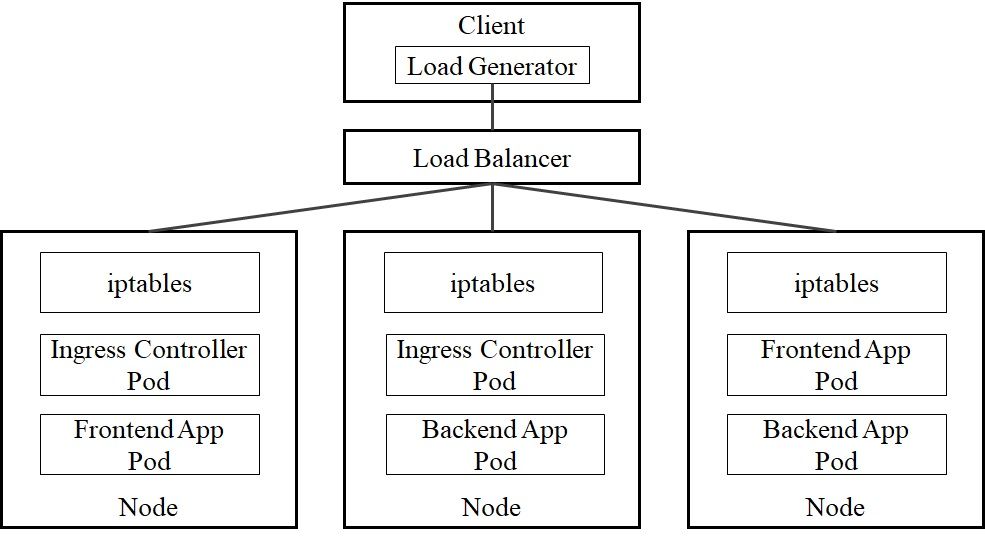
\includegraphics[clip,width=140mm]{images/exp-overall.jpg}}
    \caption{Pod削除時挙動の検証構成(要素と配置)}\label{fig10}
\end{figure}

\begin{footnotesize}
    \begin{tabularx}{\linewidth}{
            >{\hsize=0.8\hsize}X|
            >{\hsize=1.2\hsize}X
        }
        \captionsetup{font=normalsize}
        \caption{Pod削除時挙動の検証環境}\label{table5}                      \\
        要素                  & 構成                                                      \\ \hline \hline
        Kubernetes            & Microsoft Azure Kubernetes Service (v1.18.4)              \\ \hline
        Kubernetes Node VM    & Microsoft Azure Standard_F2s_v2 (2vCPU, 4GB Memory) * 3 \\ \hline
        ゲートウェイ          & NGINX Ingress Controller (Helm Chart v2.11.2)             \\ \hline
        フロントエンド        & podinfo (v4.0.6)                                          \\ \hline
        バックエンド          & podinfo (v4.0.6)                                          \\ \hline
        ロードジェネレータ    & Yandex Tank (v1.12.8)                                     \\ \hline
        ロードジェネレータ VM & Microsoft Azure Standard_F2s_v2 (2vCPU, 4GB Memory) * 1 \\ \hline
        Pod削除制御 & Litmus Chaos (v1.6.1) \\ \hline
    \end{tabularx}
\end{footnotesize}

Podを1つ削除してもクライアントへのエラー応答無く処理継続可能かを確認する.そこで,ロードジェネレータであるYandex Tank\cite{ref32}からHTTP POSTを並行数500で実行し,その間に複製されたPodの1つを削除し,応答を記録する[図\ref{fig11}].なおPodの削除にはChaos testingツールのLitmus Chaos\cite{ref33}を使い,Podのdelete APIをコールする.このAPIによりコンテナのアプリケーションにSIGTERMが送信され,続いてPodが削除される.合わせて,Podの削除とは同期せず,並行してServiceからEndpointが削除される.
\newpage
\begin{figure}[tb]
    \centerline{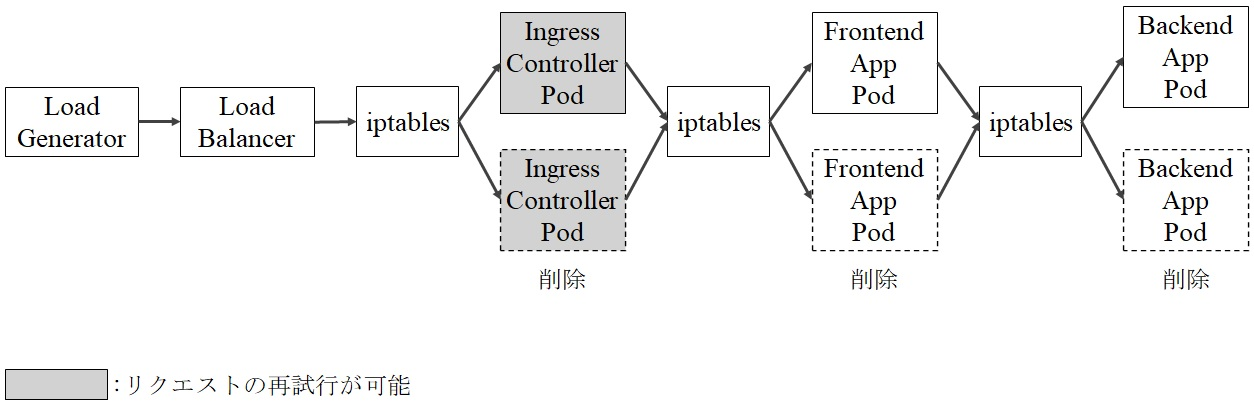
\includegraphics[clip,width=140mm]{images/exp-flow.jpg}}
    \caption{Pod削除時挙動の検証構成(フロー)}\label{fig11}
\end{figure}

なおSIGTERM受信時にNGINX Ingress Controllerは10秒間,また,podinfoは3秒間,コネクションのドレインとEndpointの削除を待つよう実装されている.加えて,NGINX Ingress Controllerは再試行と接続先の切り替え機能を持つ.つまり,この構成ではフロントエンドが一時的に利用できない場合でも再試行と切り替えを期待できる.

削除対象ごとに5回試行し,クライアントに対するエラー応答を含む試行数を表\ref{table6}に示す.

\begin{footnotesize}
    \begin{tabularx}{\linewidth}{
            >{\hsize=0.8\hsize}X|
            >{\hsize=1.2\hsize}X
        }
        \captionsetup{font=normalsize}
        \caption{Pod削除時挙動の検証結果}\label{table6} \\
        削除対象           & エラー応答を含む試行 (試行数: 5)        \\ \hline \hline
        Ingress Controller & 2                                       \\ \hline
        フロントエンド     & 0                                       \\ \hline
        バックエンド       & 2                                       \\ \hline
    \end{tabularx}
\end{footnotesize}

フロントエンドの削除ではエラー応答が無い.つまり呼び出し元であるIngress Controllerの再試行,切り替え機能が寄与している.他方,一定時間の待機のみで,再試行や切り替えを実装していない他の削除対象では,持続時間は短いがエラー応答が発生した[表\ref{table7}].エラーの発生しない試行もあり,Pod削除時の各Nodeや要素の状態に依存することがわかる.

\newpage
\begin{footnotesize}
    \begin{tabularx}{\linewidth}{
            >{\hsize=1.4\hsize}X|
            >{\hsize=0.9\hsize}X|
            >{\hsize=0.9\hsize}X|
            >{\hsize=0.9\hsize}X|
            >{\hsize=0.9\hsize}X
        }
        \captionsetup{font=normalsize}
        \caption{Pod削除時のエラー内容}\label{table7}                                      \\
        削除対象           & TCP/IP エラー数 & HTTP エラー数 & アプリケーション エラー数 & エラー持続時間(秒) \\ \hline \hline
        Ingress Controller & 5               & 0             & 0                         & 0.018              \\ \cline{2-5}
                           & 60              & 0             & 0                         & 0.279              \\ \hline
        バックエンド       & 0               & 0             & 1                         & 0.002              \\ \cline{2-5}
                           & 0               & 0             & 1                         & 0.002              \\ \hline
    \end{tabularx}
\end{footnotesize}

Ingress Controller削除時のTCP/IPエラーはコード104(ECONNRESET)と111(ECONNREFUSED)であり,クライアントであるYandex Tankが削除済みPodに対して接続を試み,RSTパケットが返された結果である.また,バックエンド削除におけるアプリケーションエラーでは,Ingress Controllerはクライアントへ正常なHTTP応答を返す一方で,ペイロードにアプリケーションからのエラーメッセージが記録されている.その内容は,フロントエンドからバックエンドに接続できないというものである.

仮定の通り,すべてのエラーの原因は,Podの削除後にiptablesルールに残った,存在しないPodへ転送を試みたことである.そして呼び出し元で再試行や切り替えなどエラー対処を行っていないケースでは,クライアントにエラー応答が返された.

高精度な時刻同期などで構成管理要素間のタイミングを合わせ,設定の非同期を原因とするエラーを解決することは可能であろう.しかしKuberetesが結果整合を受け入れて得た価値を損なう恐れがある.よってシンプルさと並行性を重視するならば,アプリケーション層での対処が望ましい.それはアプリケーション自身での実装に限らない.例えばサービスメッシュでプロキシとして使われるEnvoyは再試行機能を有する\cite{ref34}.

ところで,クラウドサービス事業者はユーザに対し,リソースが一時的に利用できない状況を前提としたアプリケーション設計(Desigin for Failure)の重要性を訴え,再試行をはじめとするデザインパターンを公開,推奨している\cite{ref35,ref36}.この考え方は故障だけでなく,利用者がリソースを共用するサービスにおいて,利用者が変化や変更作業をコントロールできない場合でも有益である.例えば,共用サーバに対する,緊急度の高い脆弱性に対するパッチ適用と再起動は,利用者がそのタイミングを管理できない代表的な例である.

このようにDesign for Failureというコンセプトは,日常的な基盤の変化に適応するためにも役立つ.同様にこの考えは,あるべき状態を維持するために基盤がリソースを再構成し続ける,宣言的構成管理においても有益である.しかしクラウドコンピューティングの文脈で使われるFailureという言葉が,データセンタ障害のような非日常的なアクシデントを連想させている印象は否めない.

なお,カオスエンジニアリングの実践について共有,議論するChaos Comminityは,カオスエンジニアリングを「不安定な状態に耐える能力をシステムが確立するための実験の規律」と定義している\cite{ref37}.不安定な状態,カオスを生み出すイベントとして障害のみが注目されがちであるが,再構成もその原因である.よって,Design for Failureにとどまらず「Design for Chaos」へと対象を広げるべきである.

アプリケーションの再構成耐性は基盤に閉じない論点であり,宣言的構成管理の将来に大きな影響を与える.よって展望の章で改めて論じる.

\section{実行空間の分離と優先制御}
KubernetesではDNSサーバなど,重要度の高いシステム要素がアプリケーションと同じNodeで動作するよう構成できる.したがって,入力時検証に加え,実行時の優先制御が求められる.不十分な優先度設定は主要なハザードシナリオであり,障害事例も多いことは,STPAによる分析[表\ref{table3}]と障害事例による評価[表\ref{table4}]から明らかである.

Kubernetesの優先制御の代表例は,OOM(Out Of Memory) Killである.優先度の低いPodを停止し,重要度の高いものを保護するポリシである.KubernetesのOOM Killは,要求(Request)と制限(Limit)の宣言値と実際の使用量によってkill対象のPodを決定する.Node全体の使用メモリ量が閾値(Eviction Policy)を超えた場合,使用量がRequestを超えたコンテナを持つPodが候補となり,Priority Classと使用量を考慮したランク付けで停止対象を決定する.障害事例による評価[表\ref{table4}]からわかる通り,OOM Killを原因としたアクシデントは多い.

宣言的構成管理のコンセプトに従い,KillされたPodは再作成される.しかし,それが新たな非安全なコントロールアクションとなり,再作成が連鎖することもある\cite{ref6}.このポリシを許容できず,アプリケーションの強制停止を回避したいユースケースもあるであろう.よって他の分離方式や優先度制御も議論されるべきである.ただし管理対象の保護が行き過ぎて利点を損なってはならない.KubernetesはNodeをいわゆるPetsではなく,容易に取り替えられるCattle\cite{ref38}として扱うことで,運用者の負担を軽減した.この割り切りは念頭に置くべきである.

\section{プルかプッシュか}
Kubernetesは各要素がAPI Serverをプルする構造を選択し,API Serverの単純化に寄与している.一方,プロセスモデル操作の起点は各要素となるため,その数に応じたAPI Serverの処理能力が必要となる.DaemonSetなど全Nodeで設定を同じにする要素で考慮が足りず,API呼び出しが自クラスタに対するDDoS攻撃となった障害事例もある[表\ref{table4}].入力時検証など他の仕組みでも解決すべき課題であるが,他領域への適用においては,規模や制御のパターンによってプッシュ型が適するケースもあるであろう.例えば,コントローラが中央集権的に順序やタイミングを制御する必要があればプッシュ型が向く.

\section{管理対象の異種混在}
KubernetesはLinuxエコシステムで開発されたため,iptablesなどLinuxカーネルの機能に強く依存しており,非Linux環境を管理対象としにくい状況が続いている.例えばMicrosoft WindowsをNodeとして利用するために,管理されるOS側でKubernetes向けの機能追加が行われている\cite{ref39}.しかしWindowsコンテナのイメージサイズが大きくコンテナ作成時間,ひいては回復時間に影響するなど,機能追加だけでは解決できない根本的な課題が残っている.

管理対象が多様であれば,そのインタフェイスを抽象化し,透過性を確保するのが従来の定石であった.しかしKubernetesは管理対象を絞り,その機能と特徴を前提に宣言的構成管理を実現した.よって適用領域の検討に際し,管理対象の多様さと抽象化は論点である.特にネットワークやストレージ領域においては管理対象が異種混在するケースが想像され,慎重な議論が必要であろう.なお,異種混在に限らない,管理対象リソースの広がりについては次章で述べる.

\chapter{展望}
宣言的構成管理の適用において,アプリケーションの再構成耐性の担保が最も重要な論点である.アプリケーションが基盤の再構成を契機とする変化に耐えられない場合には,宣言的構成管理を行う基盤の活用は難しい.一方で,アプリケーションが再構成耐性を持つのであれば,自律性を持つリソースや操作に時間がかかるリソースを管理対象にするなど,宣言的構成管理の適用範囲は広がる.この章では将来に向けた展望として,アプリケーションの再構成耐性の向上を支援する仕組みと,管理対象の広がりについて考察する.

\section{継続的検証(Continuous Verification)}
再試行など,アプリケーションに対して再構成に備える実装を行う場合,そのテストはアプリケーションの新規作成や変更後に行うだけでは十分でない.なぜなら,宣言的構成管理を行う基盤ではリソースは動的に変化を続けており,テスト時点から環境や条件が変わる可能性が高いからである.基盤やアプリケーションの設定変更,メンテナンス作業などで,リソースの状態や配置は変化する.したがって,アプリケーションは継続的にテストされるべきである.

ソフトウェアの品質管理手法の1つに,継続的インテグレーション(CI: Continuous Integration)がある\cite{ref40}.開発中のソースコードのマージと統合テストを頻繁に行うことで,問題の早期発見をはじめとする効果を期待できる.日次など定期的に,もしくはソースコードリポジトリへのチェックインなどのイベントを契機に,マージとビルド,テストを行う.また,常に本番環境に配布可能な成果物を作成する,もしくは配布まで行うアプローチをCD(Continuous Delivery)と呼ぶ\cite{ref41}.このアプローチはCIを含む.

CIは主にアプリケーションの機能要件をテストする目的で,本番と分離されたテスト環境で行われる.一方,回復性など非機能要件のテストの一部は,一般的にCIの範囲外とされる.表\ref{table8}は,Sridharanによる,分散システムにおけるテストとその実施環境,実施タイミングの例である\cite{ref42}.

\newpage
\begin{footnotesize}
    \begin{tabularx}{\linewidth}{
            >{\hsize=1.0\hsize}X|
            >{\hsize=1.0\hsize}X|
            >{\hsize=1.0\hsize}X|
            >{\hsize=1.0\hsize}X
        }
        \captionsetup{font=normalsize}
        \caption{分散システムにおけるテストと実施環境,実施タイミング}\label{table8}                                                                      \\
                             & \multicolumn{3}{|c}{Testing in production}                                             \\ \hline
        Pre-production       & Deploy                                     & Release            & Post-Relase          \\ \hline \hline
        Unit tests           & Integration tests                          & Canarying          & Teeing               \\
        Functional tests     & Tap compare                                & Monitoring         & Profiling            \\
        Component tests      & Load tests                                 & Traffic shaping    & Logs/events          \\
        Stress tests         & Shadowing                                  & Feature flagging   & Chaos testing        \\
        Fuzz tests           & Config tests                               & Exception tracking & Monitoring           \\
        Static analysis      & Soak tests                                 &                    & A/B tests            \\
        Property based tests &                                            &                    & Tracing              \\
        Coverage tests       &                                            &                    & Dynamic exploration  \\
        Benchmarking tests   &                                            &                    & Real user monitoring \\
        Regression tests     &                                            &                    & Auditing             \\
        Contract tests       &                                            &                    & On-call experience   \\
        Lint tests           &                                            &                    &                      \\
        Acceptance tests     &                                            &                    &                      \\
        Mutation tests       &                                            &                    &                      \\
        Smoke tests          &                                            &                    &                      \\
        UI/UX tests          &                                            &                    &                      \\
        Usability tests      &                                            &                    &                      \\
        Penetration tests    &                                            &                    &                      \\
        Threat modering      &                                            &                    &                      \\ \hline
    \end{tabularx}
\end{footnotesize}

Production,つまり本番環境で行われるテスト(Testing in production)が多く見られる.この背景には,規模,機能,外部環境などの観点から,分散システムにおいて本番前の環境(Pre-production)では再現が難しい,もしくは効果を得にくいテストが増えていることがある.開発から運用までのライフサイクルを時系列で表現した場合の右側でテストを行うことから,この動向は「Shift Right」と呼ばれる\cite{ref43}.

Sridharanは,Chaos testingを,本番環境において,リリース後に実施する行為と位置づけている.また,Chaos testingの先行事例で著名なNetflix社が本番環境で実践していること\cite{ref44},加えて,Chaos Comminityが公開する原則(Advanced Principles)において,本番環境での実行が強く推奨されていること\cite{ref37}から,Chaos testingは本番環境で実施してこそ価値があると認識されている.

しかし,OverOps社の調査では,本番環境で実施している回答者は全体の3\%にとどまっている\cite{ref45}.仮に影響範囲をコントロール可能としても,本番環境でChaos testingを行うリスクと懸念が背景にあるためと考察される.Chaos testingは,宣言的構成管理の適用において重要な取り組みである.したがって,本番環境での実施が難しいのであれば,本番前の環境でも実施できるよう「Shfit Left」すべきである[図\ref{fig12}].

Rosenthalらは,CIを補完,拡張するアイデアとして,アプリケーションの挙動を継続的に仮説検証するアプローチをCV(Continuous Verification)と定義している\cite{ref46}.アプリケーションやリソースのコード,構成データ変更を契機に,もしくは定期的にCVパイプラインを実行する.障害や再構成イベントを注入し動作を検証することで,アプリケーション開発者やシステム管理者は,回復性や再構成耐性に関する仮説を継続的に検証できる.
\begin{figure}[tb]
    \centerline{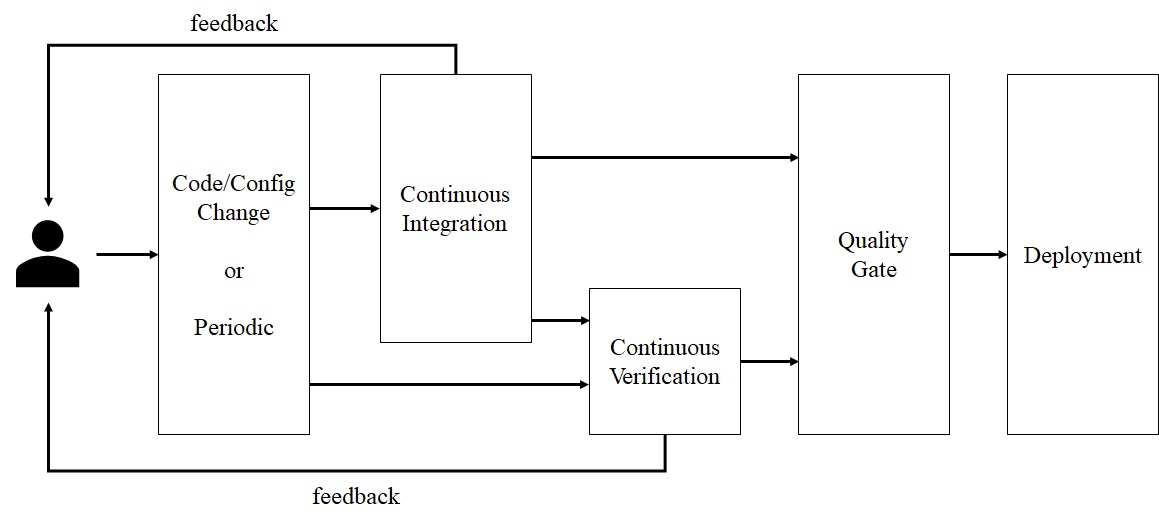
\includegraphics[clip,width=140mm]{images/cv-in-pre-production.jpg}}
    \caption{本番前環境におけるCV}\label{fig12}
\end{figure}

\subsection{Chaos testing}
CVにおけるChaos testingの実現には2つの課題がある.1つは知見のない段階では仮説検証のシナリオを作りにくいこと,もう1つは障害や再構成イベントを注入するツールは目的別に多種多様なものが存在するため,それらの統合である.

前者は仮説検証のプロセス自身が知見を得る手段であり,実践が必要である.その際には本論文のSTPAの結果などを参考とすればよい.また,後者のツール統合は,オープンソースソフトウェア開発コミュニティなどにおいて活発に議論,開発されている.\ref{sec:アプリケーションの再構成耐性}の検証で利用したLitmus Chaosはその例である.

図\ref{fig13}はLitmus Chaosの概要である.Litmus Chaosは実験(ChaosExperiment)と実行(ChaosEngine)の定義,および結果(ChaosResult)をKubernetesのカスタムリソースとして扱う.Chaos OperatorはカスタムコントローラとしてChaosEngineの投入や変更を監視し,ChaosExperimentに定義されたジョブ(Chaos Runner)を実行する.Chaos Runnerはコンテナであり,障害や再構成イベントを発生させるツールを含む.\ref{sec:アプリケーションの再構成耐性}で利用したようにKubernetes APIをコールするもの,ターゲットとするコンテナでLinuxのtcコマンド\cite{ref47}を実行しパケットロスや遅延を発生させるものなど,様々なツールを含んだExperimentが公開されている.

\newpage
\begin{figure}[tb]
  \centerline{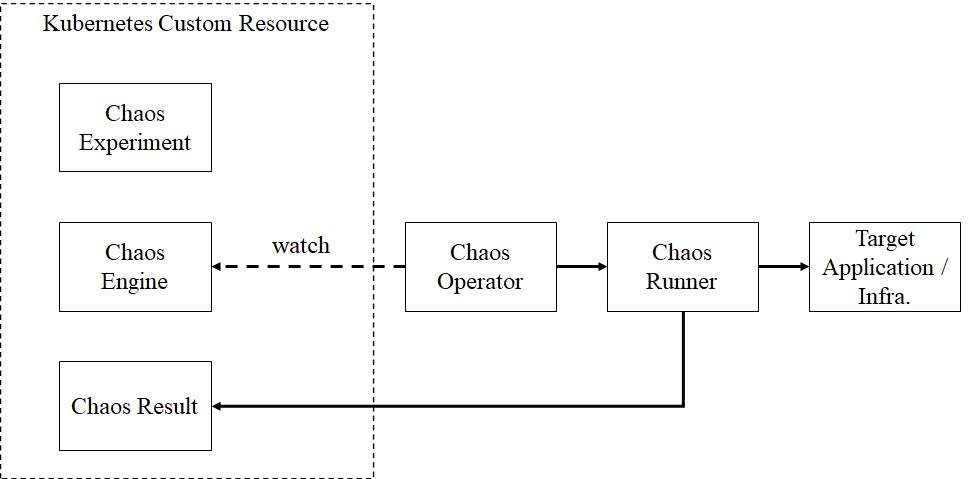
\includegraphics[clip,width=140mm]{images/litmus-overall.jpg}}
  \caption{Litmus Chaos概要}\label{fig13}
\end{figure}

ソースコード\ref{sc3}は,\ref{sec:アプリケーションの再構成耐性}で利用したPod削除検証の定義(ChaosExperiment)である."go-runner"イメージで作成したコンテナを,引数"./experiments/pod-delete"を与えて作成するよう定義している.合わせて必要な権限や既定値も定義する.

\newpage
\begin{lstlisting}[caption=Litmus Chaosの実験定義(ChaosExperiment),label=sc3]
apiVersion: litmuschaos.io/v1alpha1
description:
  message: |
    Deletes a pod belonging to a deployment/statefulset/daemonset
kind: ChaosExperiment
metadata:
  name: pod-delete
  version: 0.1.20
spec:
  definition:
    scope: Namespaced
    permissions:
      - apiGroups:
          - ""
          - "apps"
          - "batch"
          - "litmuschaos.io"
    ### snip ###
    image: "litmuschaos/go-runner:1.6.1"
    imagePullPolicy: Always
    args:
      - -c
      - ./experiments/pod-delete
    command:
      - /bin/bash
    env:
      - name: TOTAL_CHAOS_DURATION
        value: ""
      - name: RAMP_TIME
        value: ""
      - name: KILL_COUNT
        value: ""
      - name: FORCE
        value: "true"
      - name: CHAOS_INTERVAL
        value: ""
      - name: LIB_IMAGE
        value: "litmuschaos/pod-delete-helper:latest"
      - name: LIB
        value: "litmus"
    labels:
      name: pod-delete
\end{lstlisting}

そしてソースコード\ref{sc4}は,先に定義したExperimentの実行定義(ChaosEngine)である.ChaosEngineの投入や変化をChaos Operatorが検知し,Experimentを実行する.ChaosEngineには,ターゲットとなるアプリケーションや名前空間,実行時間などExperimentの実行条件を指定する.

\newpage
\begin{lstlisting}[caption=Litmus Chaosの実行定義(Engine),label=sc4]
apiVersion: litmuschaos.io/v1alpha1
kind: ChaosEngine
metadata:
  name: frontend-chaos
  namespace: podinfo
spec:
  appinfo:
    appns: "podinfo"
    applabel: "app=frontend"
    appkind: "deployment"
  annotationCheck: "false"
  engineState: "active"
  auxiliaryAppInfo: ""
  chaosServiceAccount: pod-delete-sa
  monitoring: false
  jobCleanUpPolicy: "delete"
  experiments:
    - name: pod-delete
      spec:
        components:
          env:
            - name: TOTAL_CHAOS_DURATION
              value: "15"
            - name: CHAOS_INTERVAL
              value: "30"
            - name: FORCE
              value: "false"
            - name: KILL_COUNT
              value: "1"
\end{lstlisting}

このようにChaos testingで必要となる多様なツールを統合することで,CVパイプライン内で各ツールを透過に扱うことができる.また,結果の出力も標準化されるため,後続プロセスの実行判断や開発者,管理者へのフィードバックが容易になる.このように,Chaos testingを継続的に行うのであれば,Litmus Chaosのような仕組みが望まれる.

Litmus Chaosが現時点(v.1.10.0)で公開しているKubernetes向けGeneric Experimentsの一覧と,本論文で識別したハザードシナリオとの対応を表\ref{table9}に示す.ハザードシナリオは非安全なコントロールアクションに至る原因であるが,Experimentで注入するイベントが間接的に影響するシナリオも含めた.なお,Pod単体に対するExperimentの中には対応シナリオがないものがあるが,本論文では単一障害を分析対象から除いたためであり,検証目的によっては有用である.

\newpage
\begin{footnotesize}
    \begin{tabularx}{\linewidth}{
            >{\hsize=1.0\hsize}X|
            >{\hsize=1.0\hsize}X
        }
        \captionsetup{font=normalsize}
        \caption{Litmus ChaosのExprtiment一覧とハザードシナリオとの対応}\label{table9} \\
        Experiments           & 対応するハザードシナリオ        \\ \hline \hline
        Pod Delete	& HS-2, HS-4 \\ \hline
        Pod Network Latency	& \\ \hline
        Pod Network Loss & \\ \hline
        Pod Network Corruption & \\ \hline
        Pod Network Duplication & \\ \hline
        Pod CPU Hog & 	HS-1, HS-10 \\ \hline
        Pod Memory Hog	&  HS-1, HS-10 \\ \hline
        Pod Autoscaler	& HS-2 \\ \hline
        Pod IO Stress	& HS-10 \\ \hline
        Disk Fill	& HS-10 \\ \hline
        Disk Loss	& HS-10 \\ \hline
        Node CPU Hog	& HS-1, HS-10 \\ \hline
        Node Memory Hog	& HS-1, HS-10 \\ \hline
        Node Drain	& HS-2 \\ \hline
        Node Taint	& HS-2 \\ \hline
        Node IO Stress	& HS-10 \\ \hline
        Kubelet Service Kill	& HS-5 \\ \hline
        Docker Service Kill	& HS-10 \\ \hline
        Container Kill &  \\ \hline

    \end{tabularx}
\end{footnotesize}

\section{管理対象リソースの広がり}
Kubernetesが管理対象をコンテナやサーバOS機能など軽量なリソースに絞ることで,従来の宣言的構成管理が抱えていた課題を解決したこと,また,のちにニーズの多様化を背景に,ネットワークやストレージなどに管理対象を広げていることは前述した通りである.例えば,KubernetesのServiceをクラスタ外へ公開する際に,クラウドサービスが提供するロードバランサを,クラウドサービスのAPIを通じて操作することは一般的となった\cite{ref48}.図\ref{fig8}のコントロールストラクチャで示したcloud-controller-managerが各クラウドサービスの操作を抽象化し,Kubernetesのコントローラ群であるController Manager(kube-controller-manager)と同様にControl Loopを通じてリソースの構成管理を行う.

Control Loopと,構成をコードでなくデータで定義するConfiguration as Dataという概念は,Kubernetesが宣言的構成管理を実用的にした主な理由である.そこで,その仕組みと概念を非Kubernetesリソースにも適用する動向がある.

\subsection{Kubernetesカスタムリソース/コントローラによる非Kubernetesリソースの構成管理}
Kubernetesのデザインパターンの1つに,Operatorパターン\cite{ref49}がある.Kubernetesにカスタムリソースとそれを管理するカスタムコントローラを追加し,非Kubernetesリソースであっても,Control LoopとConfiguration as Dataによる管理を実現するパターンである.従来,運用者が行っていた作業をコントローラが実現するため,Operatorパターンと呼ばれる.Operatorの適用範囲は,アプリケーションからインフラストラクチャまで幅広い\cite{ref50}.図\ref{fig14}は,仮想ネットワーク,ストレージ,データベースといった非Kubernetesリソースの構成をOperatorパターンで管理する概念図である.前述のLitmus ChaosもOperatorパターンで実装されている.Operatorには構成管理の他に,データベースのバックアップなどリソース固有の作業を実装することもある.

\begin{figure}[tb]
  \centerline{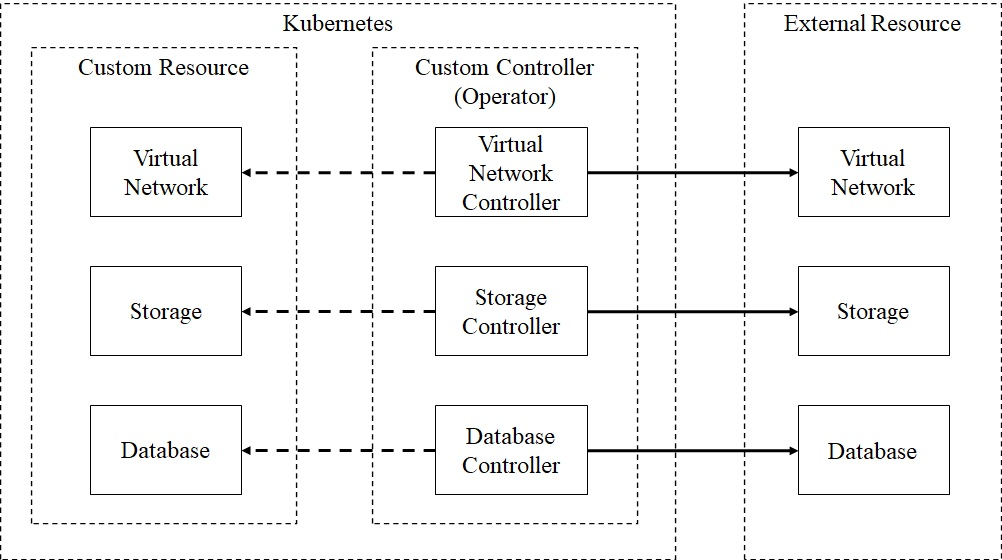
\includegraphics[clip,width=140mm]{images/operator-for-er.jpg}}
  \caption{Kubernetesカスタムリソース/コントローラによる非Kubernetesリソースの構成管理}\label{fig14}
\end{figure}

Operatorパターンの適用範囲は,Kubernetesクラスタを構成する,もしくはその上で動作するリソースに限らない.Operatorをコントロールプレーンとして,Kubernetesクラスタ外のリソースも管理できる.例えばGoolgle社のConfig Connector\cite{ref51}はGoogle Kubernetes Engineサービスのアドオン機能であるが,Google Cloudの様々なサービスやリソースの構成管理をOperatorパターンで提供している.また,Amazon Web ServicesやMicrosoft Azureなど他クラウドサービスも,提供サービスやリソースのOperatorパターンによる管理を実現するオープンソースソフトウェアプロジェクトを始めている\cite{ref52,ref53}.

ソースコード\ref{sc5}はGoolge Config Connectorでの定義例である.Kubernetesのマニフェストと同様,リソースのあるべき状態を宣言的に記述できる.

\newpage
\begin{lstlisting}[caption=Google Config Connectorの定義例(ComputeInstance),label=sc5]
apiVersion: compute.cnrm.cloud.google.com/v1beta1
kind: ComputeInstance
metadata:
  annotations:
    cnrm.cloud.google.com/allow-stopping-for-update: "true"
  name: computeinstance-sample-cloudmachine
  labels:
    created-from: "image"
    network-type: "subnetwork"
spec:
  machineType: n1-standard-1
  zone: us-west1-a
  bootDisk:
    initializeParams:
      size: 24
      type: pd-ssd
      sourceImageRef:
        external: debian-cloud/debian-9
  networkInterface:
    - subnetworkRef:
        name: computeinstance-dep-cloudmachine
      aliasIpRange:
        - ipCidrRange: /24
          subnetworkRangeName: cloudrange
  attachedDisk:
    - sourceDiskRef:
        name: computeinstance-dep1-cloudmachine
      mode: READ_ONLY
      deviceName: proxycontroldisk
      diskEncryptionKeyRaw:
        valueFrom:
          secretKeyRef:
            name: computeinstance-dep-cloudmachine
            key: diskEncryptionKey
    - sourceDiskRef:
        name: computeinstance-dep2-cloudmachine
      mode: READ_WRITE
      deviceName: persistentdisk
  minCpuPlatform: "Intel Skylake"
  serviceAccount:
    serviceAccountRef:
      name: inst-dep-cloudmachine
    scopes:
    - compute-rw
    - logging-write
\end{lstlisting}

いずれのクラウドサービスも,その取り組みにおいて多様なサービスやリソースに対応している.しかし,対象になっていない,また,制限があるサービスやリソースもあり,そこから課題が読み取れる.

中でも重要な課題は,リスク特性と影響の大きさ,リソース間の依存関係である.特に,新規作成ではなく,作成のちに定義を変更するケースが問題となる.

例えばソースコード\ref{sc5}で示したGoogle Config ConnectorによるCompuute Instance(仮想マシン)の管理では,ブートディスクに関する属性(.spec.bootDisk.initializeParams)は作成後に変更できない.よって,明示的にリソースを削除後,再作成する必要がある.これは変更の影響の大きさから,妥当な仕様である.なぜならブートディスク定義の変更によって,動作中の仮想マシンとあるべき状態の間に差が生じるが,それを埋めるためには仮想マシンの再作成が必要になるためである.仮想マシンの構成管理において,作成が短時間で済むコンテナやMicroVMと同様の再作成戦略は選択しにくい.仮想ネットワークのMTU(Maximum Transmission Unit)など,低レイヤの属性も同様である.もちろん,Kubernetesにとってコンテナがそうであったように,管理対象リソース側で技術革新があれば,状況は変わるであろう.

また,リソース間の依存関係も重要である.例えば図\ref{fig14}で挙げたデータベースを構成するための前提リソースとして,仮想ネットワークとストレージが必要と仮定する.つまり,データベースは仮想ネットワークとストレージに依存する.したがって,ネットワークやストレージの再作成が必要な変更が要求された場合,それらに依存しているデータベースの再作成も必要となりうる.

新規作成時はそれぞれのリソースのコントローラがControl Loopで依存リソースの作成完了を待てばいいが,変更時は依存関係が大きく影響する.依存関係の観点では,ネットワークの変更は特に影響範囲が大きい.その上で多くのリソースが動作しうる,つまり依存するためである.前述の仮想マシンのブートディスクと同様に,変更内容の制限など,例外的な対応が必要である.

再作成に関する時間や依存リソースの影響範囲を問題とせず,再作成を原則とする戦略も考えられる.しかしその場合,データプレーンは長時間にわたって利用不可能となりうる.リクエストの再試行などアプリケーションで解決可能な範囲を超えるケースも想定される.よって,マルチデータプレーン構成での切り替え,マイグレーションなど,さらなる考慮が必要になる.構成管理にとどまらない議論が求められるであろう.

\chapter{おわりに}

本論文では,Kubernetesの構造と事例の分析を通じ,宣言的構成管理の適用可能性と論点を導いた.宣言的構成管理において,構成管理機能はリソース管理の主導権を有し,宣言を満たすようリソースの再構成を動的,非同期に行う.したがって,アプリケーションはそれに耐えうる設計と実装,運用を行うべきである.基盤の構成要素やレイヤに閉じた議論で部分最適に陥らず,アプリケーション,その開発と検証プロセスを含めた全体最適の視点を持つことが重要である.

\section{本研究の成果}
はじめに第2章で本研究に関連する先行研究とその課題を整理し,Kubernetesがそれらをどのように解決したかを述べた.第3章では,STPAを用いたKuberntesの安全性,構造分析を行い,アクシデントにつながるハザードシナリオを識別した.第4章では,識別したハザードシナリオを障害事例によって分類し,その妥当性を評価した.第5章では,分析によって得られた構造上の特徴をもとに,宣言的構成管理を分散コンピューティング基盤へ適用する際に検討すべき論点や課題を述べた.第6章は,第5章の論点を踏まえ,宣言的構成管理の将来に向けた展望を考察した.

\section{本研究の社会的な意義}
Kubernetesは既成概念にとらわれないアイデアを多く取り入れた,また,構成要素の多い複雑な基盤ソフトウェアである.従来の基盤との違いを理解して利用しなければ,価値が引き出せないだけでなく,リスクを負いかねない.しかし,その構造と特徴を,安全性の観点から分析した文献は少ない.Kubernetesはエコシステムの著しい成長を背景に,今後も採用例が増加すると考えられる.コントロールストラクチャやハザードシナリオなど,本論文の成果はリスク評価や問題解決,カオスエンジニアリングの一助となるであろう.

また,宣言的構成管理の適用を主題として導いた論点であるが,クラウドコンピューティングの文脈でも有用である.特にアプリケーションの再構成耐性は,クラウドコンピューティングの利用においても意識すべきである.故障という非日常のイベントだけでなく,再構成という日常的なイベントを意識することは,その準備を行う強い動機付けとなる.

\section{本研究の学術的な意義}
宣言的構成管理はKubernetesやクラウドサービスでの実装が先行しており,アカデミアにおいて研究が活発とは言いにくい状況である.そのため,本論文で参考にした2010年前後の先行研究から,現在に至るまでの,この領域での知の繫がりや積み上げが乏しい.本論文は先行研究の課題をKubernetesがいかに解決したかを整理,考察し,現状の論点と展望を示すことで,そのギャップを埋める貢献となった.

\chapter*{謝辞}
本研究と論文執筆にあたり,主指導教員として終始ご指導賜りました篠田陽一教授に心より御礼申し上げます.研究テーマのみならず,様々なテクノロジや研究,考え方をご紹介いただき,研究者としての視野を広げることができました.また,副指導教員である知念賢一教授,副研究テーマをご担当いただいた宇多仁助教にも,ご指導に深く感謝いたします.

次に,篠田研究室の皆さまにも深謝しております.特に,多様な背景と動機を持ち,働きながら研究を続ける東京サテライトの皆さまと机を並べることは,大いに刺激となりました.また,修了生の皆さまにも多くのアドバイスをいただき,御礼申し上げます.特に阿部博博士には,研究室に入るきっかけを作っていただいただけでなく,節目で貴重なご助言をいただきました.学会で論文を臆することなく発表できたのは,明るく背中を押していただいたお陰です.

また,働きながら研究することにご理解くださった,日本マイクロソフト株式会社の皆さまにも深く感謝いたします.特にマネージャである飯島徹さまからは,社会人学生のご経験から暖かいお言葉をいただき,励みになりました.

そして何より,家族に感謝します.働きながら研究するためには,相応の好奇心や情熱,行動力が必要でした.それを育んでくれた両親には感謝の言葉しかありません.最後に,学びたいという気持ちを理解,尊重し,支えてくれた妻に心から感謝します.

重ねて,皆さまへ深く感謝の意を表し,謝辞といたします.

\chapter*{本研究に関する発表論文}
\section*{国内会議(査読あり)}
\begin{itemize}
    \item 真壁徹,篠田陽一,”分散コンピューティング基盤における宣言的構成管理の適用可能性と論点”,インターネットと運用技術シンポジウム論文集,volume 2020,pp 17-24, 情報処理学会(2020).
\end{itemize}

\renewcommand{\bibname}{参考文献}
\begin{thebibliography}{99}
    \bibitem{ref1} Liu, C., Loo, B.T., Mao, Y.: Declarative automated cloud resource orchestration, Proc. SoCC ’11, No.26, pp.1-8, ACM(2011).
    \bibitem{ref2} Ansible, https://docs.ansible.com (参照 2020-08-13).
    \bibitem{ref3} Terraform, https://www.terraform.io (参照 2020-08-13).
    \bibitem{ref4} Imperative vs Declarative, https://dominik-tornow.medium.com/imperative-vs-declarative-8abc7dcae82e (参照 2020-12-07).
    \bibitem{ref5} Burns, B., Grant, B., Oppenheimer, D., et al: Borg, omega, and Kubernetes, Comm. ACM, Vol.59, No.5, pp.50-57(2016).
    \bibitem{ref6} Kubernetes Failure Stories, https://github.com/hjacobs/kubernetes-failure-stories (参照 2020-08-13).
    \bibitem{ref7} Bozóki, S., Szalontai, J., Pethő, D., et al: Application of extreme value analysis for characterizing the execution time of resilience supporting mechanisms in Kubernetes, Proc. EDCC ’20, pp.185-199, Springer(2020).
    \bibitem{ref8} CNCF: CNCF SURVEY 2020.
    \bibitem{ref9} Chen, X., Mao, Y., Mao, Z.M., et al: Declarative configuration management for complex and dynamic networks, Proc. Co-NEXT ’10, No.6, pp.1-12, ACM(2010).
    \bibitem{ref10} Loo, B.T., Condie, T., Garofalakis, M., et al: Declarative networking: language, execution and optimization. Proc. SIGMOD '06, pp.97-108, ACM(2006).
    \bibitem{ref11} Warren, D.H.D., Pereira, L.M. and Pereira, F.: Prolog – the language and its im- plementation compared with Lisp, Proc. 1977 Symposium on Artificial Intelligence and Programming Languages, pp.109–115, ACM(1977).
    \bibitem{ref12} Morris, K.: Infrastructure as Code, 2nd Edition, O'Reilly Media(2020).
    \bibitem{ref13} Mao, M. and Humphrey, M.: A performance study on the VM startup time in the cloud, Proc. CLOUD '12, pp.423-430, IEEE(2012).
    \bibitem{ref14} Ceri, S., Gottlob, G. and Tanca, L.: What you always wanted to know about Data- log (and never dared to ask), IEEE Trans. Knowledge and Data Engineering, Vol.1, No.1, pp.146–166, IEEE(1989).
    \bibitem{ref15} Ryzhyk, R. and Budiu, M.: Differential Datalog, VMware Research(2019).
    \bibitem{ref16} Gunawi, H.S.,Hao, M., Suminto, R.O., et al: Why does the cloud stop computing? Lessons from hundreds of service outages. Proc. SoCC '16, pp.1-16, ACM(2016).
    \bibitem{ref17} The Mechanics of Kubernetes, https://dominik-tornow.medium.com/the-mechanics-of-kubernetes-ac8112eaa302 (参照 2020-11-29).
    \bibitem{ref18} CNI, https://github.com/containernetworking (参照 2020-11-29).
    \bibitem{ref19} Container Storage Interface, https://github.com/container-storage-interface (参照 2020-11-29).
    \bibitem{ref20} Xavier, B., Ferreto, T. and Jersak, L.: Time provisioning evaluation of kvm docker and unikernels in a cloud platform. Proc. CCGrid ’16, pp.277-280, IEEE(2016).
    \bibitem{ref21} Agache, A., Brooker, M., Florescu, A., et al: Firecracker: Lightweight Virtualization for Serverless Applications. Proc. NSDI ’20, Usenix(2020).
    \bibitem{ref22} Assigning Pods to Nodes, https://kubernetes.io/docs/concepts/scheduling-eviction/assign-pod-node/ (参照 2020-12-08).
    \bibitem{ref23} Burns, B.: How Kubernetes Changes Operations, login Usenix Mag., Vol.40, Usenix(2015).
    \bibitem{ref24} Schwarzkopf, M., Konwinski, M., Abd-El-Malek, M., et al: Omega: flexible, scalable schedulers for large compute clusters, Proc. EuroSys '13. pp. 351-364, ACM(2013).
    \bibitem{ref25} I do declare! Infrastructure automation with Configuration as Data, https://cloud.google.com/blog/products/containers-kubernetes/understanding-configuration-as-data-in-kubernetes (参照 2020-12-10).
    \bibitem{ref26} Leveson, N.G.: Engineering A Safer World: Systems Thinking Applied to Safety, MIT Press(2011).
    \bibitem{ref27} Leveson, N.G. and Thomas, J P.: STPA HANDBOOK(2018).
    \bibitem{ref28} Leveson, N.G. and Thomas, J P., Shirasaka, S. (Translators into Japanese), et al.: STPA HANDBOOK 日本語版 Ver.0.2(2018).
    \bibitem{ref29} Open Policy Agent, https://github.com/open-policy-agent (参照 2020-08-13).
    \bibitem{ref30} NGINX Ingress Controller, https://github.com/kubernetes/ingress-nginx (参照2020-08-13).
    \bibitem{ref31} podinfo, https://github.com/stefanprodan/podinfo (参照 2020-08-13).
    \bibitem{ref32} Yandex Tank, https://github.com/yandex/yandex-tank (参照 2020-12-11).
    \bibitem{ref33} Litmus, https://github.com/litmuschaos/litmus (参照 2020-12-11).
    \bibitem{ref34} envoy: How do I handle transient failures?, https://www.envoyproxy.io/docs/envoy/latest/faq/load\_balancing/transient\_failures (参照 2020-08-13).
    \bibitem{ref35} Running Containerized Microservices on AWS. Design for Failure, https://docs.aws.amazon.com/whitepapers/latest/running-containerized-microservices/design-for-failure.html (参照 2020-12-09).
    \bibitem{ref36} Azure Application Architecture Guide, https://docs.microsoft.com/en-us/azure/architecture/guide/ (参照 2020-12-09).
    \bibitem{ref37} PRINCIPLES OF CHAOS ENGINEERING, https://principlesofchaos.org/ (参照 2020-12-10).
    \bibitem{ref38} Tilkov, S.: The modern cloud-based platform, IEEE Software, Vol. 32, No.2, pp. 112-116, IEEE(2015).
    \bibitem{ref39} Built-in Support for Kubernetes – What's new in Windows Server 2019, https://docs.microsoft.com/en-us/windows-server/get-started-19/whats-new-19\#built-in-support-for-kubernetes (参照 2020-08-13).
    \bibitem{ref40} Andres, C.: Extreme Programming Explained: Embrace Change, Second Edition, Addison-Wesley Professional(2004).
    \bibitem{ref41} Chen, L.: Continuous Delivery: Huge Benefits, but Challenges Too, IEEE Software, Vol. 32, No.2, pp. 50-54, IEEE(2015).
    \bibitem{ref42} Sridharan, C.: Distributed Systems Observability, O'Reilly Media(2018).
    \bibitem{ref43} Friese, S.: Testing the Unexpected: A Shift Right in DevOps Testing, https://www.stickyminds.com/article/testing-unexpected-shift-right-devops-testing (参照 2020-12-10).
    \bibitem{ref44} Basiri, A., Hochstein, L., Jones, et al: Automating Chaos Experiments in Production, Proc. ICSE-SEIP '19. pp. 31-40, IEEE(2019).
    \bibitem{ref45} The State of Software Quality, OverOps(2020).
    \bibitem{ref46} Rosenthal, C., Jones, N.: Chaos Engineering, O'Reilly Media(2020).
    \bibitem{ref47} tc(8) — Linux manual page, https://man7.org/linux/man-pages/man8/tc.8.html (参照 2020-12-10).
    \bibitem{ref48} Kubernetes - Service Type LoadBalancer, https://kubernetes.io/docs/concepts/services-networking/service/\#loadbalancer (参照 2020-12-10).
    \bibitem{ref49} Operator pattern, https://kubernetes.io/docs/concepts/extend-kubernetes/operator/ (参照 2020-12-10).
    \bibitem{ref50} OperatorHub.io, https://operatorhub.io/ (参照 2020-12-10).
    \bibitem{ref51} Config Connector overview, https://cloud.google.com/config-connector/docs/overview (参照 2020-12-10).
    \bibitem{ref52} AWS Controllers for Kubernetes (ACK), https://github.com/aws/aws-controllers-k8s (参照 2020-12-10).
    \bibitem{ref53} Azure Service Operator (for Kubernetes), https://github.com/Azure/azure-service-operator (参照 2020-12-10).
\end{thebibliography}
\end{document}
